\section{Implementation and Evaluation}\label{sec:implementation}
%\subsection{Implementation}
\begin{figure}[t]
	\centering
	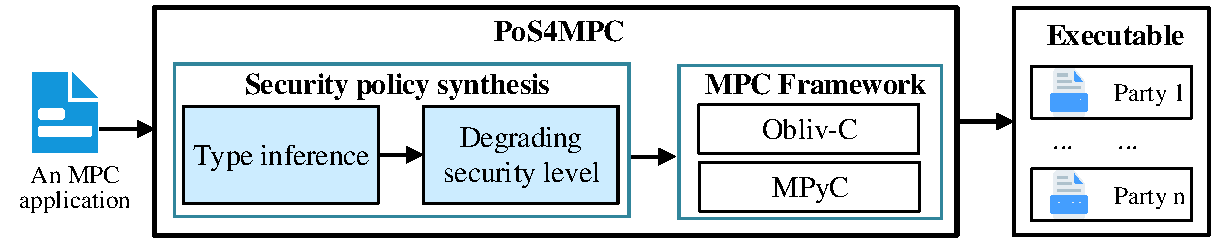
\includegraphics[scale=0.56]{img/workflow-v1}
	\vspace{-2mm}
	\caption{The workflow of our tool \TNAME}
	\label{fig-impl}
	\vspace{-3mm}
\end{figure}
We have implemented our approach in a tool, named \TNAME. The workflow of \TNAME is shown in Fig.~\ref{fig-impl},
The input is an MPC program in C, which is parsed %the C program to construct its
to an intermediate representation (IR)
inside the LLVM Compiler~\cite{llvm} where call graph and control flow graphs are constructed %via LLVM passes
at the LLVM IR level.
We then perform the type inference which computes
the a perfect security policy for the given program.
To be accurate, we perform a field-sensitive pointer
analysis~\cite{BalatsourasS16} and our type inference is also field-sensitive.
As the next step, we leverage the KLEE symbolic execution engine~\cite{CadarDE08}
to explore all the feasible symbolic executions, as well as the symbolic
values of the return variable and secret branching variables of each symbolic execution.
Based on them, we iteratively check if a secret branching variable % specified by the security policy
can be declassified.  %until no more can be declassified, during which
If it is the case, its security level %of the found secret branching variable
is degraded and the result is fed back to the type inference to refine security levels before checking the next secret branching variable.
%in the security policy if it does not compromise security.
After that, we transform the program into the input of Obliv-C~\cite{ZahurE15} by which the program can be compiled into
executable implementations, one for each party. Obliv-C is an extension of C for implementing 2-party MPC applications using Yao's garbled circuit protocol~\cite{yao82}.
For experimental purposes, \TNAME also features the high-level MPC framework MPyC~\cite{MPyC20},
which is a Python package for implementing $n$-party MPC applications ($n\geq 1$) using Shamir's secret sharing protocol~\cite{Shamir79}.
The C program is transformed into Python by a translator~\cite{C2Python}.

We also implement an optimization in our tool to alleviate the path explosion problem. Instead of directly checking the validity of $\Psi_x(t,t')$
for each secret branching variable $x$ and pair of symbolic executions $t$ and $t'$,
we first check if the premise $\phi\wedge \Primed(\phi')\wedge e=\Primed(e')$
of $\Psi_x(t,t')$ is satisfiable. We can conclude that $\Psi_x(t,t')$ is valid for any secret branching variable $x$ if the premise $\phi\wedge \Primed(\phi')\wedge e=\Primed(e')$ is unsatisfiable.
Furthermore, this yields a sound compositional reasoning approach which allows to split
a program into a sequence of function calls. When each pair of the symbolic executions
for each function cannot result in the same return value, we can conclude that
$\Psi_x(t,t')$ is valid for any secret branching variable $x$ and any pair of symbolic executions $t$ and $t'$
of the entire program.


%
% automatic verification tool \TNAME based on the symbolic engine KLEE.
%Figure \ref{fig-impl} shows the workflow of \TNAME.
%Fortunately, the symbolic and concrete variables give a fine mapping to secret and public variables.
%We simplify the implementation of \TNAME by regarding symbolic variables as secret variables, and concrete values as public data.
%The input of \TNAME is the program $p$.
%The collector of \TNAME fully explores all reachable paths of the given program to extract the conditions.
%\TNAME constructs the leakage lower bound and the leakage of the given program and then generates queries of the constraint solver to accomplish verification.
%\TNAME will output a hint indicating the insecure case if the program fails the verification.

\subsection{Evaluation Setup}\label{sec:experiments}
%In this section, we evaluate the efficiency and effectiveness of our approach and the performance improvement of
%MPC applications with our security policies.


%
%\smallskip
%\noindent
%{\bf Benchmarks.}
For an evaluation of our approach, we conduct experiments on five typical 2-party MPC applications~\cite{benchmarks}, i.e.,
quicksort ({\tt QS})~\cite{mpcqsort}, linear search ({\tt LinS})~\cite{absent}, binary search  ({\tt BinS})~\cite{absent},
  almost search ({\tt AlmS})~\cite{Knuth73},
and  private set intersection  ({\tt PSI})~\cite{Andreea21}.
%Taking a private array $\vec{a}_i$ of integers from each party $\Party{i}$ as input,
%which forms one array $\vec{a}$ where the first half is $\vec{a}_1$
%and the second half is $\vec{a}_2$,
{\tt QS} outputs the list of indices of a given integer array $\vec{a}$ in its ordered version, where
the first half of $\vec{a}$ is given by one party and the second half of $\vec{a}$ is given by the another party.
{\tt LinS} (resp. {\tt BinS} and {\tt AlmS}) outputs the index
of an integer $b$ in an array $\vec{a}$ if it exists, $-1$ otherwise, where
the integer array $\vec{a}$ is the input from one party and the integer $b$ is the input from
the another party.
{\tt LinS} always scans the array from the start to the end even though it has found the integer $b$.
{\tt BinS} is a standard iterative approach on a sorted array, where the array index is protected via oblivious read access machine~\cite{GoldreichO96}.
{\tt AlmS} is a variant of {\tt BinS}, where the input array is almost sorted, namely,
each element is at either the correct position or the closest neighbour
of the correct position.
{\tt PSI} outputs the intersection of two integer sets, each of which
is an input from one party.

All the experiments were conducted on a desktop with 64-bit Linux Mint 20.1, Intel Core i5-6300HQ CPU, 2.30 GHz and 8 GB RAM. When evaluating MPC applications, the client of each party
is executed with a single thread.
%The speedup is calculated by the formula $std \ time/opt \ time$.
%The measurement result is the average of 10 times repetitions.


\subsection{Performance of Security Policy Synthesis}
{\bf Security policy}.
The results of our approach is shown in Table~\ref{table:policyresults},
where column (LOC) shows the number of lines of code,
column (\#Branch var) shows the number of branching variables
while column (\#Other var) shows the number of other variables,
columns (After TS) and (After Check) respectively
show the number of secret branching variables after
applying the type system and checking if the secret branching variables can be declassified,
columns (Before refinement) and (After refinement) respectively show
the number of other secret variables before and after refining the type inference by feeding
back the results of the symbolic reasoning.
(Note that the input variables are excluded in counting.)

We can observe that only few variables (2 for \texttt{QS}, 1 for \texttt{LinS}, 2 for \texttt{BinS}, 2 for \texttt{AlmS} and 2 for \texttt{PSI})
can be found to be public by solely using the type system.
With our symbolic reasoning approach, more secret branching variables can be declassified
without compromising the security (3 for \texttt{QS}, 1 for \texttt{LinS}, 1 for \texttt{BinS}, 2 for \texttt{AlmS} and 1 for \texttt{PSI}).
After refining the type inference using results of the symbolic reasoning approach,
more secret variables can be declassified (2 for \texttt{QS}, 1 for \texttt{LinS} and 2 for \texttt{PSI}).
Overall, our approach annotates 2, 1, 7, 12 and 1 internal variables as secret out of
10, 4, 10, 16 and 6 variables for \texttt{QS}, \texttt{LinS}, \texttt{BinS}, \texttt{AlmS} and \texttt{PSI}, respectively.
%
%Our security policy synthesis securely declassifies 3 (resp. 1, 1, 1, 1) secret conditions at
%{\tt QS}'s Line 17, 21, 31 (resp. {\tt LinS}'s Line 9, {\tt BinS}'s Line 30, {\tt AlmS}'s Line 29, {\tt PSI}'s Line 9), while {\tt QS} (resp. {\tt LinS}, {\tt BinS}, {\tt AlmS}, {\tt PSI})
%contains 3 (resp. 1, 2, 6, 1) secret conditions. In detail,
%{\tt QS} declassifies the comparisons of the pivot and array elements,
%{\tt LinS} (resp. {\tt PSI}) declassifies the equality of the search value and array elements,
%{\tt BinS} (resp. {\tt AlmS}) declassifies the equality of the search value and array's boundary value in each iteration.
%Furthermore, with declassifing above secret conditions, the partition result of {\tt QS} become public so that no secret indexes for array access.
%The {\tt LinS} (resp. {\tt BinS}, {\tt AlmS}) can early return its result once it find the search value.
%The {\tt PSI} can jump to next loop round once it find a intersection value. Overall, {\tt QS} (resp. {\tt LinS}, {\tt BinS}, {\tt AlmS}, {\tt PSI}) reduces more computations, not only the secret conditional branches.
%

\smallskip
\noindent
{\bf Execution time}. The execution time of our approach is shown in Table~\ref{table:policytime},
where columns (SE) and (Check) respectively show the execution time (in second unless indicated by h for hour) of collecting symbolic executions
and checking if secret branching variables can be declassified, by varying
the size of the input array for each program from 10 to 100 with step 10.
We did not report the execution time of our type system, as
it is less than 0.1 second for each benchmark.

\begin{table}[t]
    \centering
    \scalebox{0.8}{
    \begin{tabular}{|c|c|c|c|c|c|c|c|}
    \hline
    \multirow{2}{*}{\bf Name} & \multirow{2}{*}{\bf LOC} & \multirow{2}{*}{\bf \#Branch var} & \multirow{2}{*}{\bf \#Other var}& \multicolumn{2}{c|}{\bf \#Secret branch var} & \multicolumn{2}{c|}{\bf \#Other secret var} \\     \cline{5-8}                                                                                                                                                                                                                                                                                                                                   &            &                                       &   & After TS & After Check  & Before refinement & After refinement\\ \hline
   {\bf QS}    & 56  & 4 & 6  &  3 & 0    & 4  & 2    \\ \hline
   {\bf LinS}  & 25  & 1 & 3  &  1 & 0    & 2  & 1   \\ \hline
   {\bf BinS}  & 46  & 2 & 8  &  2 & 1    & 6  & 6     \\ \hline
   {\bf AlmS}  & 73  & 6 & 10 &  6 & 4    & 8  & 8      \\ \hline
   {\bf PSI}   & 34  & 1 & 5  &  1 & 0    & 3  & 1 \\ \hline
    \end{tabular}
    }
    \caption{Number of (secret) branching variables}
    \label{table:policyresults}\vspace{-6mm}
\end{table}

\begin{table}[t]
\centering
    \scalebox{0.65}{
    \begin{tabular}{|c|cccccccccccccccccccc|}
    \hline
    \multirow{3}{*}{\bf Name}  & \multicolumn{20}{c|}{\bf  Length}                                                                                                                                                                                                                                                                                                                                                 \\ \cline{2-21}
                         & \multicolumn{2}{c|}{10}             & \multicolumn{2}{c|}{20}            & \multicolumn{2}{c|}{30}            & \multicolumn{2}{c|}{40}             & \multicolumn{2}{c|}{50}             & \multicolumn{2}{c|}{60}             & \multicolumn{2}{c|}{70}             & \multicolumn{2}{c|}{80}             & \multicolumn{2}{c|}{90}             & \multicolumn{2}{c|}{100} \\ \cline{2-21}
                            & {SE}    & \multicolumn{1}{c|}{Check} & {SE}   & \multicolumn{1}{c|}{Check} & {SE}   & \multicolumn{1}{c|}{Check} & {SE}    & \multicolumn{1}{c|}{Check} & {SE}    & \multicolumn{1}{c|}{Check} & {SE}    & \multicolumn{1}{c|}{Check} & {SE}    & \multicolumn{1}{c|}{Check} & {SE}    & \multicolumn{1}{c|}{Check} & {SE}    & \multicolumn{1}{c|}{Check} & {SE}         & {Check}      \\ \hline
   {\bf QS}                  & 11.6 & \multicolumn{1}{c|}{0.8}   & 0.4h & \multicolumn{1}{c|}{304.2} & 2.0h & \multicolumn{1}{c|}{959.8} & 5.0h  & \multicolumn{1}{c|}{0.6h}   & 9.5h  & \multicolumn{1}{c|}{0.9h}   & 15.5h & \multicolumn{1}{c|}{1.3h}   & 22.6h & \multicolumn{1}{c|}{1.6h}   & 31.0h & \multicolumn{1}{c|}{2.0h}   & 40.7h & \multicolumn{1}{c|}{2.3h}   & 51.6h      & 2.7h        \\ \hline
   {\bf LinS}                  & 0.4  & \multicolumn{1}{c|}{1.0}   & 0.6 & \multicolumn{1}{c|}{1.0}   & 1.0 & \multicolumn{1}{c|}{1.0}   & 1.4  & \multicolumn{1}{c|}{1.0}   & 2.0  & \multicolumn{1}{c|}{1.1}   & 2.6  & \multicolumn{1}{c|}{1.1}   & 3.4  & \multicolumn{1}{c|}{1.2}   & 4.2  & \multicolumn{1}{c|}{1.2}   & 5.2  & \multicolumn{1}{c|}{1.3}   & 6.2       & 1.4        \\ \hline
   {\bf BinS}                 & 0.8  & \multicolumn{1}{c|}{1.1}   & 2.1 & \multicolumn{1}{c|}{4.3}   & 3.8 & \multicolumn{1}{c|}{10.2}  & 6.4  & \multicolumn{1}{c|}{20.0}  & 9.5  & \multicolumn{1}{c|}{34.8}  & 13.8 & \multicolumn{1}{c|}{54.6}  & 19.5 & \multicolumn{1}{c|}{80.1}  & 25.6 & \multicolumn{1}{c|}{103.4} & 34.1 & \multicolumn{1}{c|}{151.4} & 42.7      & 204.7      \\ \hline
   {\bf AlmS}                 & 1.3  & \multicolumn{1}{c|}{0.8}   & 4.3 & \multicolumn{1}{c|}{3.5}   & 7.7 & \multicolumn{1}{c|}{10.0}  & 14.1 & \multicolumn{1}{c|}{18.6}  & 20.6 & \multicolumn{1}{c|}{32.3}  & 28.9 & \multicolumn{1}{c|}{51.0}  & 40.7 & \multicolumn{1}{c|}{77.4}  & 55.1 & \multicolumn{1}{c|}{110.3} & 74.9 & \multicolumn{1}{c|}{148.2} & 94.4      & 200.0      \\ \hline
   {\bf PSI}                  & 1.7  & \multicolumn{1}{c|}{0.5}   & 4.3 & \multicolumn{1}{c|}{1.0}   & 8.0 & \multicolumn{1}{c|}{1.5}   & 13.2 & \multicolumn{1}{c|}{2.1}   & 20.0 & \multicolumn{1}{c|}{2.8}   & 28.6 & \multicolumn{1}{c|}{3.5}   & 39.3 & \multicolumn{1}{c|}{4.3}   & 50.9 & \multicolumn{1}{c|}{5.3}   & 63.0 & \multicolumn{1}{c|}{6.4}   & 79.6      & 7.8        \\ \hline
    \end{tabular}
    }
    \caption{Execution time of our security policy synthesis approach}
    \label{table:policytime}
  \vspace{-7mm}
\end{table}

%\begin{table}[t]
%    \scalebox{0.62}{
%    \begin{tabular}{|c|c|c|ccccccccccccccccccc|}
%    \hline
%    \multirow{3}{*}{\bf Name}  & \multirow{3}{*}{\bf TS} & \multicolumn{20}{c|}{\bf  Length}                                                                                                                                                                                                                                                                                                                                                 \\ \cline{3-22}
%                          &         & \multicolumn{2}{c|}{10}             & \multicolumn{2}{c|}{20}            & \multicolumn{2}{c|}{30}            & \multicolumn{2}{c|}{40}             & \multicolumn{2}{c|}{50}             & \multicolumn{2}{c|}{60}             & \multicolumn{2}{c|}{70}             & \multicolumn{2}{c|}{80}             & \multicolumn{2}{c|}{90}             & \multicolumn{2}{c|}{100} \\ \cline{3-22}
%                          &          & {SE}    & \multicolumn{1}{c|}{Check} & {SE}   & \multicolumn{1}{c|}{Check} & {SE}   & \multicolumn{1}{c|}{Check} & {SE}    & \multicolumn{1}{c|}{Check} & {SE}    & \multicolumn{1}{c|}{Check} & {SE}    & \multicolumn{1}{c|}{Check} & {SE}    & \multicolumn{1}{c|}{Check} & {SE}    & \multicolumn{1}{c|}{Check} & {SE}    & \multicolumn{1}{c|}{Check} & {SE}         & {Check}      \\ \hline
%   {\bf QS}               & 0.049               & 11.6 & \multicolumn{1}{c|}{0.8}   & 0.4h & \multicolumn{1}{c|}{304.2} & 2.0h & \multicolumn{1}{c|}{959.8} & 5.0h  & \multicolumn{1}{c|}{0.6h}   & 9.5h  & \multicolumn{1}{c|}{0.9h}   & 15.5h & \multicolumn{1}{c|}{1.3h}   & 22.6h & \multicolumn{1}{c|}{1.6h}   & 31.0h & \multicolumn{1}{c|}{2.0h}   & 40.7h & \multicolumn{1}{c|}{2.3h}   & 51.6h      & 2.7h        \\ \hline
%   {\bf LinS}              & 0.044               & 0.4  & \multicolumn{1}{c|}{1.0}   & 0.6 & \multicolumn{1}{c|}{1.0}   & 1.0 & \multicolumn{1}{c|}{1.0}   & 1.4  & \multicolumn{1}{c|}{1.0}   & 2.0  & \multicolumn{1}{c|}{1.1}   & 2.6  & \multicolumn{1}{c|}{1.1}   & 3.4  & \multicolumn{1}{c|}{1.2}   & 4.2  & \multicolumn{1}{c|}{1.2}   & 5.2  & \multicolumn{1}{c|}{1.3}   & 6.2       & 1.4        \\ \hline
%   {\bf BinS}             & 0.048               & 0.8  & \multicolumn{1}{c|}{1.1}   & 2.1 & \multicolumn{1}{c|}{4.3}   & 3.8 & \multicolumn{1}{c|}{10.2}  & 6.4  & \multicolumn{1}{c|}{20.0}  & 9.5  & \multicolumn{1}{c|}{34.8}  & 13.8 & \multicolumn{1}{c|}{54.6}  & 19.5 & \multicolumn{1}{c|}{80.1}  & 25.6 & \multicolumn{1}{c|}{103.4} & 34.1 & \multicolumn{1}{c|}{151.4} & 42.7      & 204.7      \\ \hline
%   {\bf AlmS}            & 0.062               & 1.3  & \multicolumn{1}{c|}{0.8}   & 4.3 & \multicolumn{1}{c|}{3.5}   & 7.7 & \multicolumn{1}{c|}{10.0}  & 14.1 & \multicolumn{1}{c|}{18.6}  & 20.6 & \multicolumn{1}{c|}{32.3}  & 28.9 & \multicolumn{1}{c|}{51.0}  & 40.7 & \multicolumn{1}{c|}{77.4}  & 55.1 & \multicolumn{1}{c|}{110.3} & 74.9 & \multicolumn{1}{c|}{148.2} & 94.4      & 200.0      \\ \hline
%   {\bf PSI}              & 0.048               & 1.7  & \multicolumn{1}{c|}{0.5}   & 4.3 & \multicolumn{1}{c|}{1.0}   & 8.0 & \multicolumn{1}{c|}{1.5}   & 13.2 & \multicolumn{1}{c|}{2.1}   & 20.0 & \multicolumn{1}{c|}{2.8}   & 28.6 & \multicolumn{1}{c|}{3.5}   & 39.3 & \multicolumn{1}{c|}{4.3}   & 50.9 & \multicolumn{1}{c|}{5.3}   & 63.0 & \multicolumn{1}{c|}{6.4}   & 79.6      & 7.8        \\ \hline
%    \end{tabular}
%    }
%    \caption{Execution time of our security policy synthesis approach}
%    \label{Table:results}
%    \centering
%\end{table}

%
%\BEGIN{TABLE}[T]
%    \SCALEBOX{0.6}{
%    \BEGIN{TABULAR}{|C|C|C|CCCCCCCCCCCCCCCCCCCC|}
%    \HLINE
%    \MULTIROW{3}{*}{\BF nAME} & \MULTIROW{3}{*}{\BF  loc} & \MULTIROW{3}{*}{\BF ts} & \MULTICOLUMN{20}{C|}{\BF  lENGTH}                                                                                                                                                                                                                                                                                                                                                 \\ \CLINE{4-23}
%                          &                        &                     & \MULTICOLUMN{2}{C|}{10}             & \MULTICOLUMN{2}{C|}{20}            & \MULTICOLUMN{2}{C|}{30}            & \MULTICOLUMN{2}{C|}{40}             & \MULTICOLUMN{2}{C|}{50}             & \MULTICOLUMN{2}{C|}{60}             & \MULTICOLUMN{2}{C|}{70}             & \MULTICOLUMN{2}{C|}{80}             & \MULTICOLUMN{2}{C|}{90}             & \MULTICOLUMN{2}{C|}{100} \\ \CLINE{4-23}
%                          &                        &                     & {se}    & \MULTICOLUMN{1}{C|}{cHECK} & {se}   & \MULTICOLUMN{1}{C|}{cHECK} & {se}   & \MULTICOLUMN{1}{C|}{cHECK} & {se}    & \MULTICOLUMN{1}{C|}{cHECK} & {se}    & \MULTICOLUMN{1}{C|}{cHECK} & {se}    & \MULTICOLUMN{1}{C|}{cHECK} & {se}    & \MULTICOLUMN{1}{C|}{cHECK} & {se}    & \MULTICOLUMN{1}{C|}{cHECK} & {se}    & \MULTICOLUMN{1}{C|}{cHECK} & {se}         & {cHECK}      \\ \HLINE
%   {\BF qs}                    & 64                     & 0.049               & 11.6 & \MULTICOLUMN{1}{C|}{0.8}   & 0.4H & \MULTICOLUMN{1}{C|}{304.2} & 2.0H & \MULTICOLUMN{1}{C|}{959.8} & 5.0H  & \MULTICOLUMN{1}{C|}{0.6H}   & 9.5H  & \MULTICOLUMN{1}{C|}{0.9H}   & 15.5H & \MULTICOLUMN{1}{C|}{1.3H}   & 22.6H & \MULTICOLUMN{1}{C|}{1.6H}   & 31.0H & \MULTICOLUMN{1}{C|}{2.0H}   & 40.7H & \MULTICOLUMN{1}{C|}{2.3H}   & 51.6H      & 2.7H        \\ \HLINE
%   {\BF lINs}               & 27                     & 0.044               & 0.4  & \MULTICOLUMN{1}{C|}{1.0}   & 0.6 & \MULTICOLUMN{1}{C|}{1.0}   & 1.0 & \MULTICOLUMN{1}{C|}{1.0}   & 1.4  & \MULTICOLUMN{1}{C|}{1.0}   & 2.0  & \MULTICOLUMN{1}{C|}{1.1}   & 2.6  & \MULTICOLUMN{1}{C|}{1.1}   & 3.4  & \MULTICOLUMN{1}{C|}{1.2}   & 4.2  & \MULTICOLUMN{1}{C|}{1.2}   & 5.2  & \MULTICOLUMN{1}{C|}{1.3}   & 6.2       & 1.4        \\ \HLINE
%   {\BF bINs}                 & 53                     & 0.048               & 0.8  & \MULTICOLUMN{1}{C|}{1.1}   & 2.1 & \MULTICOLUMN{1}{C|}{4.3}   & 3.8 & \MULTICOLUMN{1}{C|}{10.2}  & 6.4  & \MULTICOLUMN{1}{C|}{20.0}  & 9.5  & \MULTICOLUMN{1}{C|}{34.8}  & 13.8 & \MULTICOLUMN{1}{C|}{54.6}  & 19.5 & \MULTICOLUMN{1}{C|}{80.1}  & 25.6 & \MULTICOLUMN{1}{C|}{103.4} & 34.1 & \MULTICOLUMN{1}{C|}{151.4} & 42.7      & 204.7      \\ \HLINE
%   {\BF aLMs}                  & 80                     & 0.062               & 1.3  & \MULTICOLUMN{1}{C|}{0.8}   & 4.3 & \MULTICOLUMN{1}{C|}{3.5}   & 7.7 & \MULTICOLUMN{1}{C|}{10.0}  & 14.1 & \MULTICOLUMN{1}{C|}{18.6}  & 20.6 & \MULTICOLUMN{1}{C|}{32.3}  & 28.9 & \MULTICOLUMN{1}{C|}{51.0}  & 40.7 & \MULTICOLUMN{1}{C|}{77.4}  & 55.1 & \MULTICOLUMN{1}{C|}{110.3} & 74.9 & \MULTICOLUMN{1}{C|}{148.2} & 94.4      & 200.0      \\ \HLINE
%   {\BF psi}                   & 36                     & 0.048               & 1.7  & \MULTICOLUMN{1}{C|}{0.5}   & 4.3 & \MULTICOLUMN{1}{C|}{1.0}   & 8.0 & \MULTICOLUMN{1}{C|}{1.5}   & 13.2 & \MULTICOLUMN{1}{C|}{2.1}   & 20.0 & \MULTICOLUMN{1}{C|}{2.8}   & 28.6 & \MULTICOLUMN{1}{C|}{3.5}   & 39.3 & \MULTICOLUMN{1}{C|}{4.3}   & 50.9 & \MULTICOLUMN{1}{C|}{5.3}   & 63.0 & \MULTICOLUMN{1}{C|}{6.4}   & 79.6      & 7.8        \\ \HLINE
%    \END{TABULAR}
%    }
%    \CAPTION{eXECUTION TIME OF OUR SECURITY POLICY SYNTHESIS APPROACH}
%    \LABEL{tABLE:SPS}
%    \CENTERING
%\END{TABLE}

We can observe that our symbolic reasoning approach is able to check
all the secret branching variables in few minutes (up to 294.4s)
except for {\tt QS}.
After an in-depth analysis, we found that the number of symbolic executions is exponential in the length
of the input array for {\tt QS} and {\tt PSI}
while it is linear in the length of the input array for the other benchmarks.
Our compositional reasoning approach works very well
on {\tt PSI}, otherwise it would take similar execution time
as on {\tt QS}. Indeed, a loop of {\tt PSI} is implemented as a sequence of function calls each of which has a fixed number of symbolic executions.
Furthermore, each pair of symbolic executions in the called function cannot result in the same return value.
Therefore, the number of symbolic executions and the execution time of our symbolic reasoning approach is reduced significantly.
However, our compositional reasoning approach does not work
on {\tt QS}. Although the number of symbolic executions grows exponentially on {\tt QS},
the execution time of checking if secret branching variables can be declassified
is still reduced by our optimization, which avoids the checking of the constraint $\Psi_x(t,t')$
if its premise $\phi\wedge \Primed(\phi')\wedge e=\Primed(e')$ is unsatisfiable.


%
%
%As the result, the security policy synthesis of QS (resp. LinS, BinS, AlmS, PSI) takes 19.0h (resp. 3.8s, 82.2s, 99.3s, 34.2s) on average.
%QS takes significantly more time due to the path explosion problem, the number of execution paths of QS is factorial to its input array size.
%The number of execution paths of LinS (resp. BinS, AlmS) is linear to its input array size.
%But BinS (resp. AlmS) contains more branches and assumptions about the input than LinS.
%Thus, the symbolic execution of BinS (resp. AlmS) takes more time to determine the reachability of a new path when exploring program paths.
%To avoid PSI's exponential number of execution paths,
%we unroll PSI's bounded loop and split PSI into a sequence of function calls as PSI calls linear scan per loop.
%We verified each function call cannot result in the same return value.
%Therefore, the SE and Verify of PSI are much faster than QS. We have also optimized the QS policy synthesis.
%To fully explore QS's execution path, there are O(n2) calls of the partition function.
%However, most partition calls have the same input array length except the values of arrays are different.
%We verify every possible partition call with different lengths in {\tt QS}, and verified any partition call cannot result in the same state of {\tt QS}'s output.
%Above optimization eliminates duplicate symbolic execution and only needs $O(n)$ times of partition calls.
%Although we mitigate the path explosion problem of {\tt QS}, we cannot fully eliminate it due to the partition process's path explosion problem.
%
%Our security policy synthesis securely declassifies 3 (resp. 1, 1, 1, 1) secret conditions at
%{\tt QS}'s Line 17, 21, 31 (resp. {\tt LinS}'s Line 9, {\tt BinS}'s Line 30, {\tt AlmS}'s Line 29, {\tt PSI}'s Line 9), while {\tt QS} (resp. {\tt LinS}, {\tt BinS}, {\tt AlmS}, {\tt PSI})
%contains 3 (resp. 1, 2, 6, 1) secret conditions. In detail,
%{\tt QS} declassifies the comparisons of the pivot and array elements,
%{\tt LinS} (resp. {\tt PSI}) declassifies the equality of the search value and array elements,
%{\tt BinS} (resp. {\tt AlmS}) declassifies the equality of the search value and array's boundary value in each iteration.
%Furthermore, with declassifing above secret conditions, the partition result of {\tt QS} become public so that no secret indexes for array access.
%The {\tt LinS} (resp. {\tt BinS}, {\tt AlmS}) can early return its result once it find the search value.
%The {\tt PSI} can jump to next loop round once it find a intersection value. Overall, {\tt QS} (resp. {\tt LinS}, {\tt BinS}, {\tt AlmS}, {\tt PSI}) reduces more computations, not only the secret conditional branches.
%


\subsection{Performance Improvement of MPC Applications}
To evaluate the performance improvement of the MPC applications,
we compare the execution time (in second), the size of the circuits (in $10^6\times$gates), and
the volume of communication traffic (in MB) of each benchmark with the security policies v1 and v2,
where v1 is obtained by solely applying our type system
and v2 is obtained from v1 by degrading security levels and refinement
without compromising the security.
The measurement results are given as the average of 10 times repetitions in order to minimize
noises.

\begin{figure}[t]
    \centering
    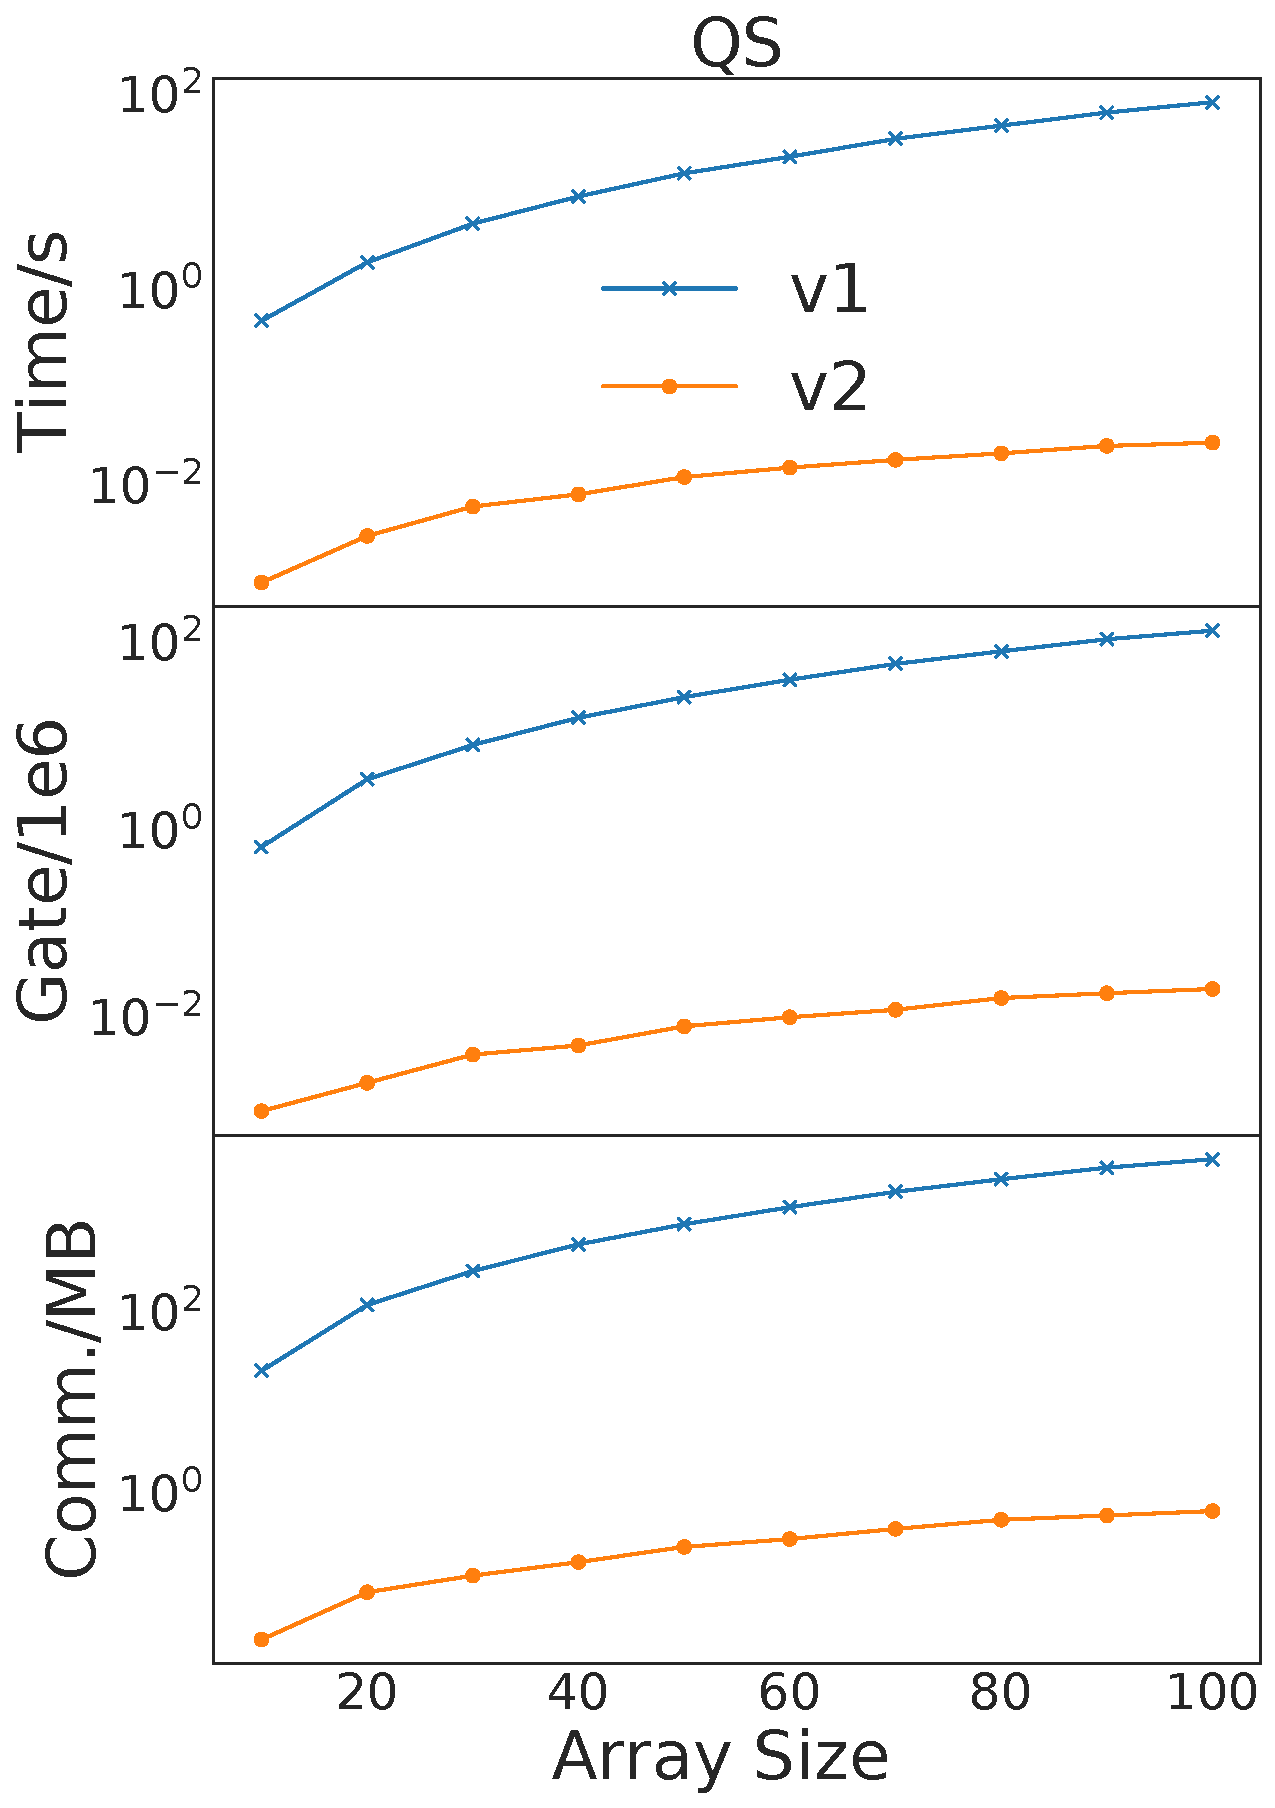
\includegraphics[width=0.24\textwidth]{img/gc100Left}
    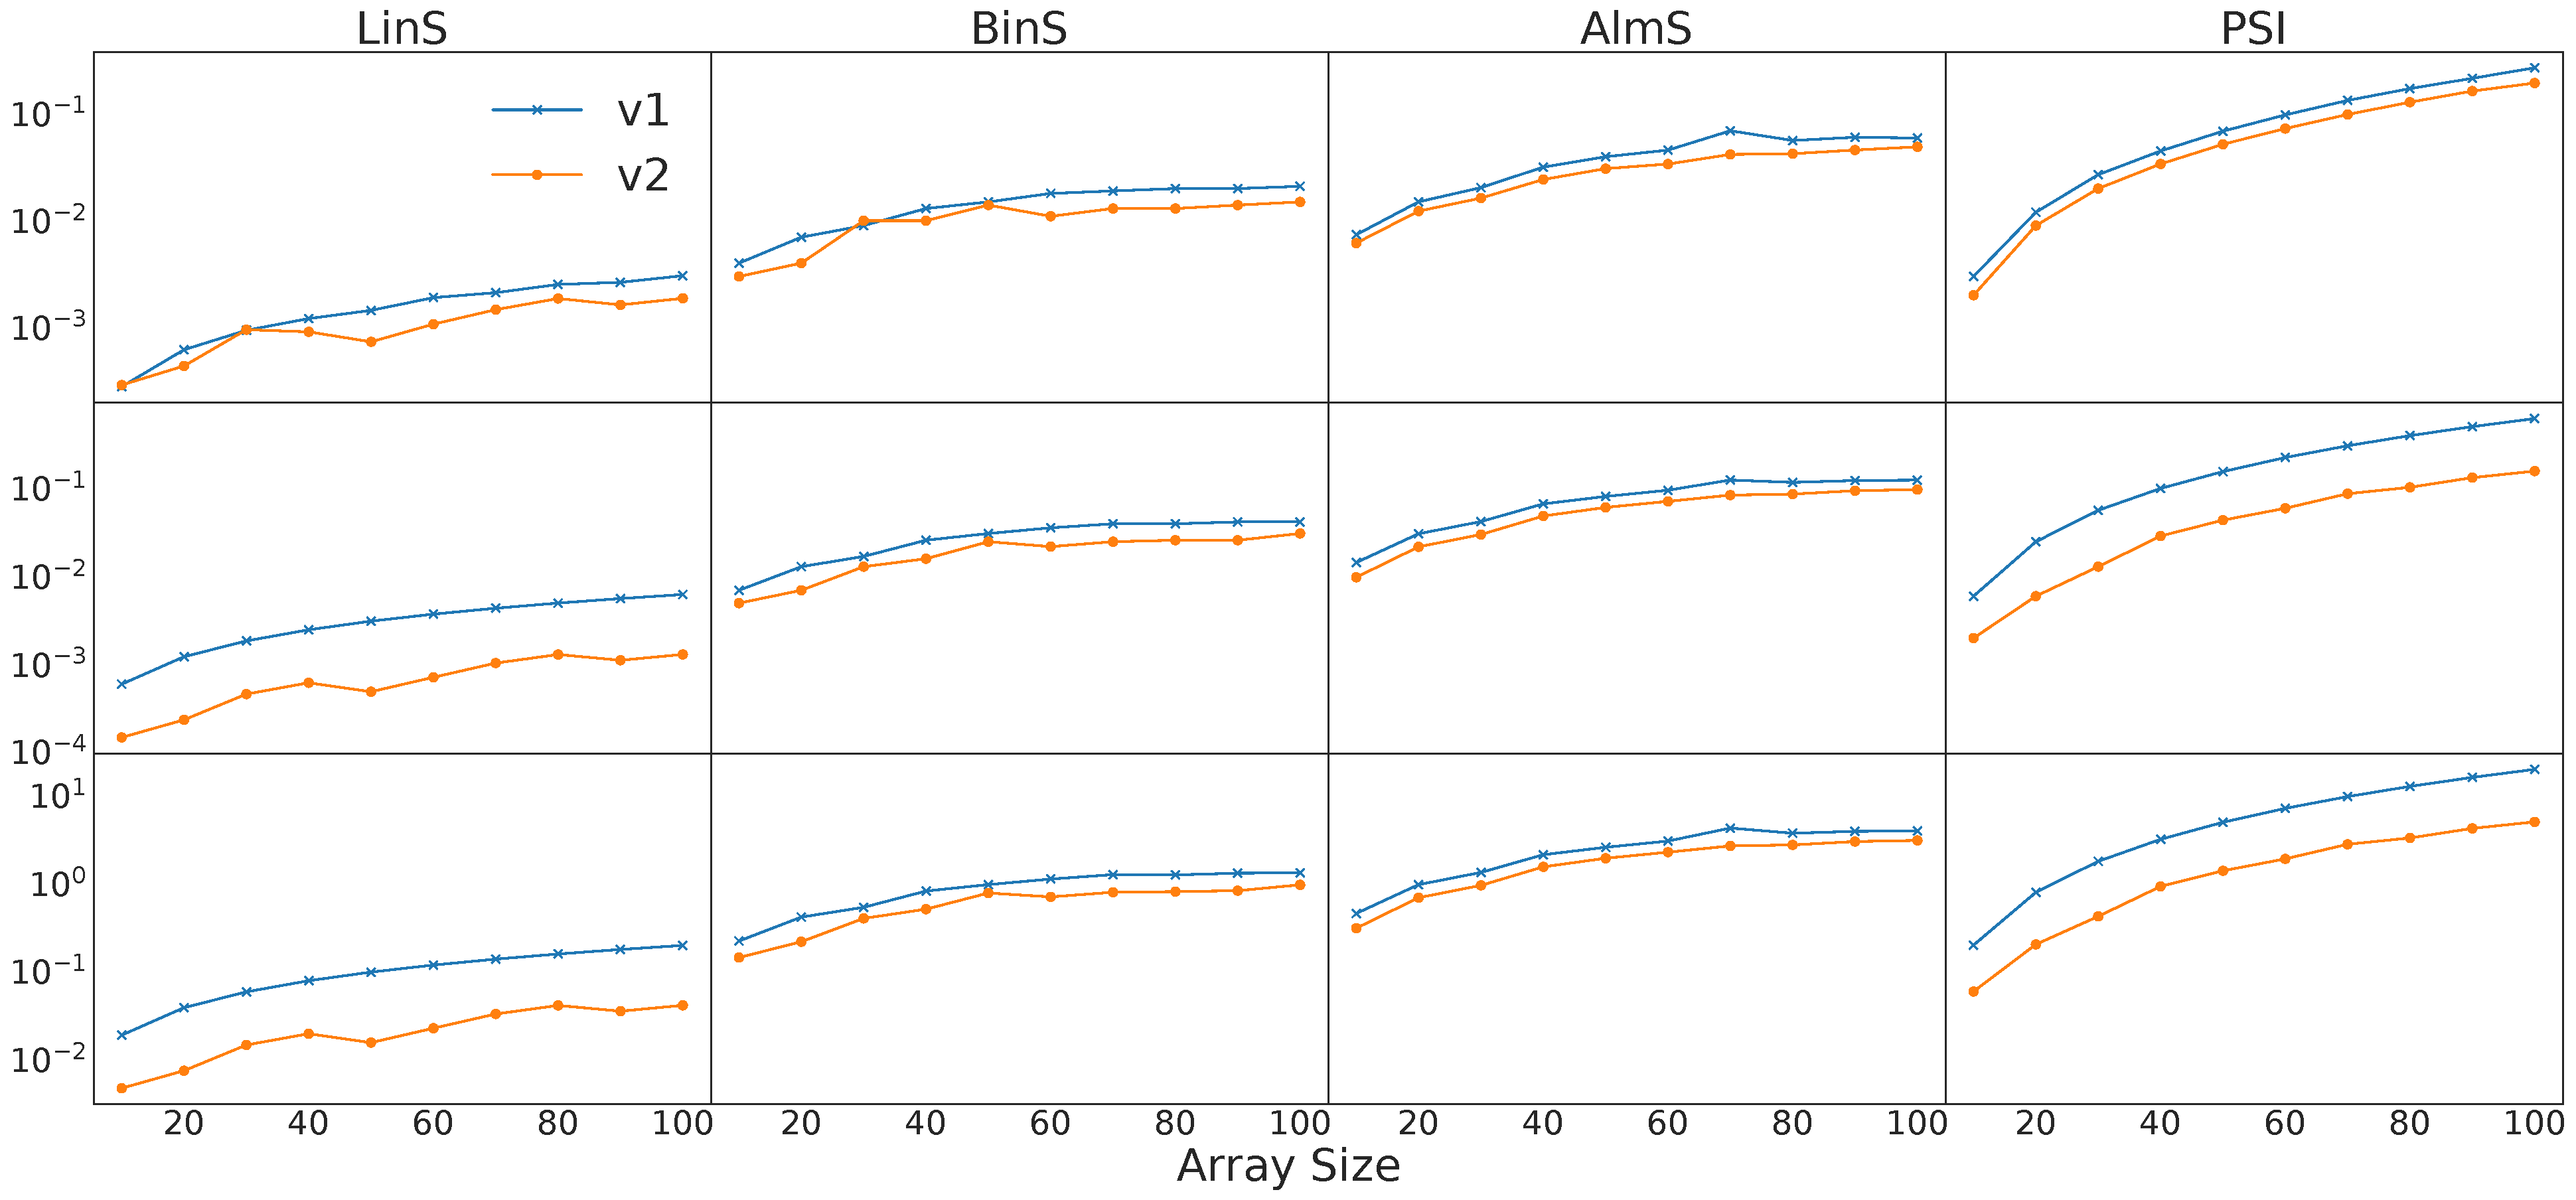
\includegraphics[width=0.74\textwidth]{img/gc100Right}
    \vspace{-1mm}
    \caption{Execution time (Time) in second, the number of gates (Gate) in 1e6 gates, Communication (Comm.) in MB using Obliv-C}
    \label{fig:gc}  \vspace{-2mm}
\end{figure}

\smallskip
\noindent
{\bf By Obliv-C.} The results in Obliv-C are depicted in Fig.~\ref{fig:gc}, where
the size of the random input array for each benchmark varies from 10 to 100 with step 10.
Overall, we can observe that the performance improvement is significant, in particular,
on {\tt QS}.
%
In detail, compared over the security policy v1 on {\tt QS} (resp. {\tt LinS}, {\tt BinS}, {\tt AlmS}, and {\tt PSI}),
on average, the security policy v2 reduces (1) the execution time by $1.56\times 10^5\%$ (resp. $45\%$, $38\%$, $31\%$ and $36\%$),
(2) the size of circuits by $3.61\times 10^5\%$ (resp. $368\%$, $52\%$, $38\%$ and $275\%$),
and (3) the volume of communication traffic by $4.17\times 10^5\%$ (resp. $367\%$, $53\%$, $39\%$ and $274\%$).
This demonstrates the performance improvement of the MPC applications
in  Obliv-C that uses Yao's garbled circuit protocol.

\begin{figure}[t]
    \centering
    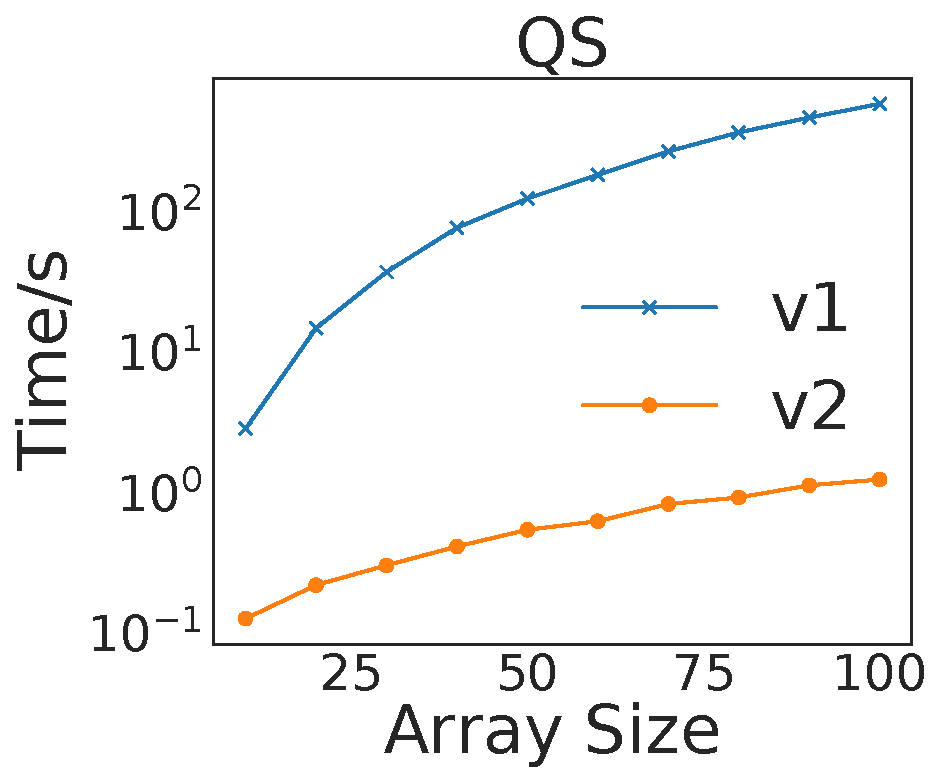
\includegraphics[width=0.24\textwidth]{img/ss100Left}
    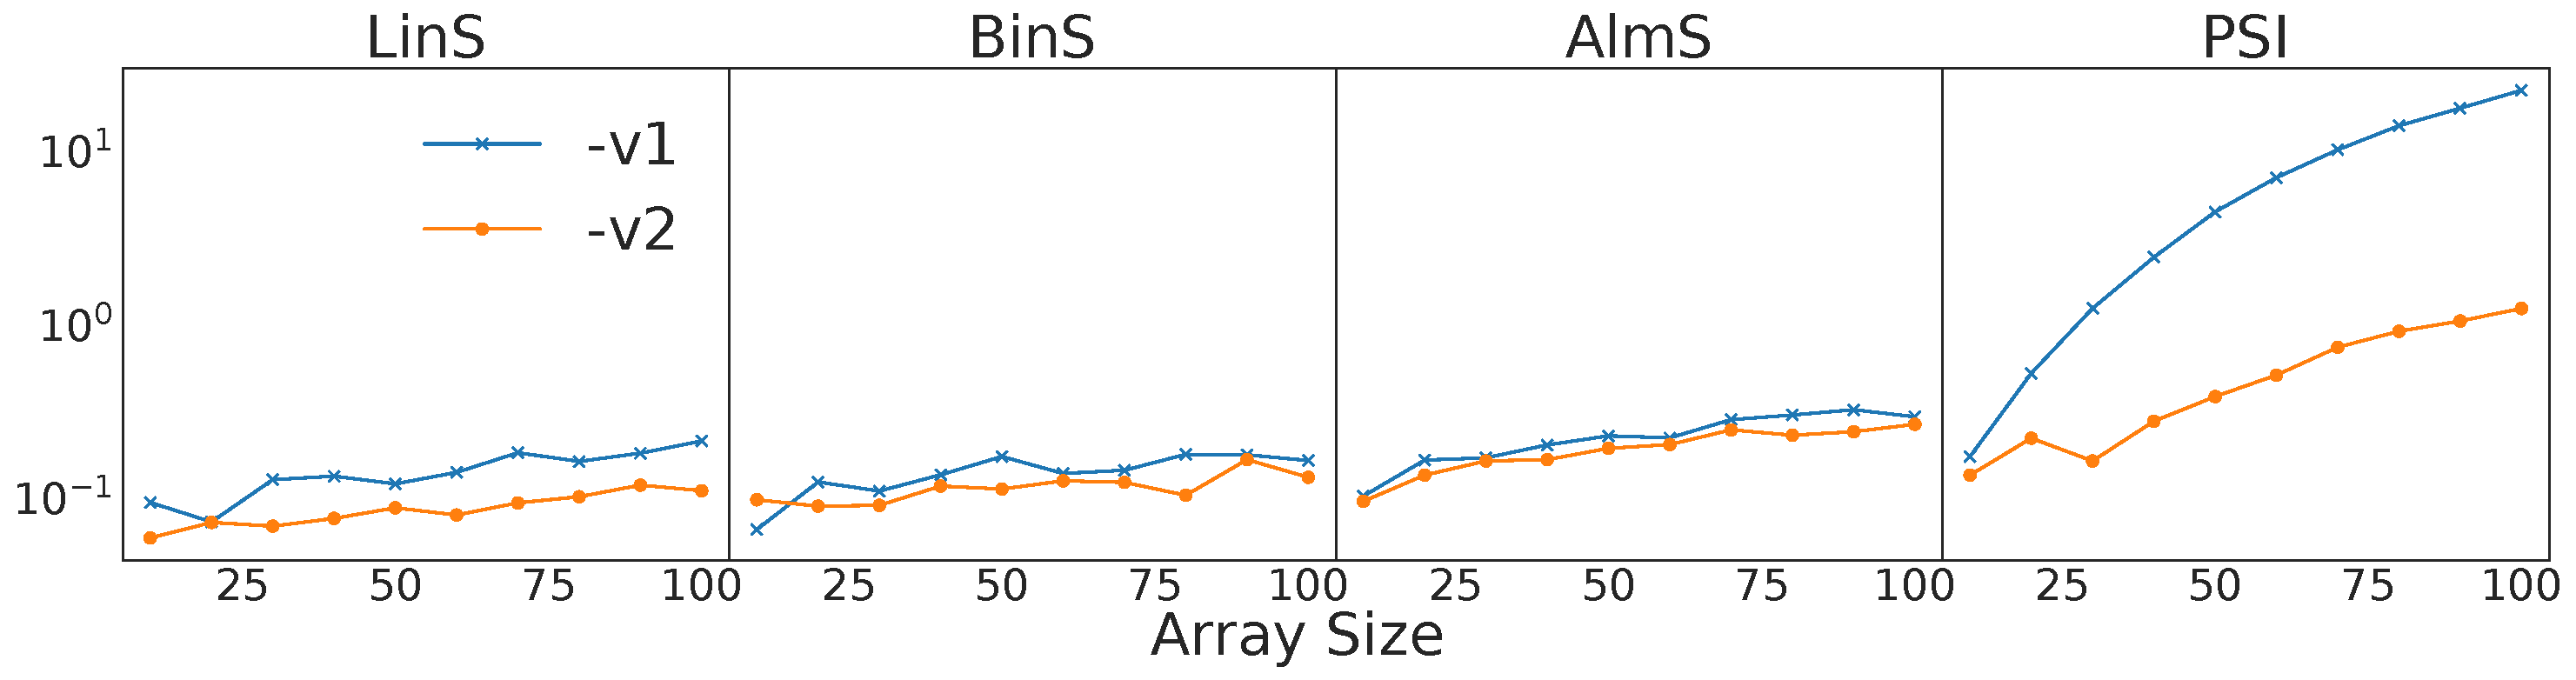
\includegraphics[width=0.7515\textwidth]{img/ss100Right}
   \vspace{-5mm} \caption{Execution time (Time) in second using MPyC}
    \label{fig:ss}  \vspace{-4mm}
\end{figure}

\smallskip
\noindent
{\bf By MPyC.} The results in MPyC are depicted in Fig.~\ref{fig:ss}.
Since  MPyC does not provide the size of circuits and the volume of communication traffic, we only report
execution time in Fig.~\ref{fig:ss}.
The results show that degrading security levels also improves execution time
in MPyC that uses Shamir's secret sharing protocol.
Compared over the security policy v1 on benchmark {\tt QS} (resp. {\tt LinS}, {\tt BinS}, {\tt AlmS}, and {\tt PSI}), on average the security policy v2 reduces the execution time by $2.5\times 10^4\%$ (resp. $64\%$, $23\%$, $17\%$ and $996\%$).


\begin{comment}

\smallskip
\noindent
{\bf Comparing with Batcher Bitonic sorting.}


We experiment our optimization approach and verification tool on 6 pairs of study cases.
The experiment result shows that our verification tool verifies a program within seconds.
Our optimization approach reduces 25\% to 91\% circuit size and communications and achieves 1.25$\times$ to 3.84$\times$ performance speedup in Yao's garbled circuit protocol, 1.25$\times$ to 24.14$\times$ speedup in Shamir's secret sharing protocol.


\subsubsection{Environment setting}
All of our experiments are implemented on a Linux desktop with 2.30 GHz CPU and 8 GB memory.
We run clients of parties on the same machine with a single thread for each client.
The speedup is calculated by the formula $std \ time/opt \ time$.
The measurement result is the average of 10 times repetitions.

We fully implement all study case programs in two real-world MPC frameworks: Obliv-C and MPyC.
Obliv-C implements Yao's garbled circuit protocol.
MPyC implements Shamir's secret sharing protocol.
We survey many MPC frameworks for our experiments.
It is disappointing that we cannot implement our all study cases on frameworks \cite{spdz,aby2,sharemind}.
They compile the whole circuit before protocol execution.
So we cannot use runtime information to avoid useless computations in them.


\subsubsection{Study cases}
To our knowledge, no program set contains many MPC application implementations.
So we collect six programs as study cases from the literature and open source project \cite{ZahurE15,absent,mpcqsort}.
We optimize the programs by our strategy and verify their leakage security.
All opt programs are verified that they are leakage secure.
We call the original version of a study case program as std and the optimized version of a study case program as opt.

The first study case is MPC sorting.
The sorting program receives two private integer arrays and outputs the ordered indexes of each array item.
We compare our optimized sorting program with the state-of-the-art MPC sorting program.
The std program is an implementation of Batcher sort that is the most popular sorting algorithm in MPC applications.
The opt program is an implementation of quicksort.
An oblivious quicksort has seriously poor performance due to the oblivious of control flow.
We optimize oblivious quicksort to a significant improvement.
Our optimization is similar to \cite{mpcqsort} but without the random shuffle because we prove its security.

The MPC searching study case searches an integer in an array and outputs its index if found.
The group of searching programs has three different algorithms.
Linear search is a commonly used algorithm in MPC programs.
The std program scans the array from the start to the end even though it has found the element.
Our opt program reveals the comparison result of the std.
Once the opt finds the element, it terminates immediately.
Binary search is a standard iterative implementation.
The std program accesses array items by oblivious index,
so it uses oblivious RAM to avoid leaking oblivious index.
Our opt program reveals the result of the equality test and terminates once it finds the element.
Almost Search is a variant of Binary Search.
The inputs of the almost search program are almost in order.
An item of the almost ordered array may be at the correct position, or the positions left or right next to the correct position.
The implementation of std and optimization of opt is similar to binary search.

The quadratic PSI computes the intersection of two privacy sets.
% Optimized OT-based PSI protocols \cite{pssz} perform much better than general MPC protocols.
We adopt a naive implementation of PSI to illustrate the effect of our method in the general MPC program.
The opt program reveals the result of the items' equality test.
Once the opt program finds two identical elements, it ignores the remaining comparisons and jumps to the next round to search for the next element.

Line segment intersection program is an application of MPC in computational graphics.
It receives two line segments and outputs the intersection point coordinate if they intersect.
The computation between line segments is float point which is much more expensive than integers in MPC.
Our opt program terminates if two line segments do not intersect while the std program always computes a point by the intersection point formula.
\subsubsection{Verification Result}
\begin{table}[ht]
    \centering
    \caption{Verification Detail}
    \setlength{\tabcolsep}{1mm}
    \begin{tabular}{c|c|c|c|c}
    \hline
    Program           & Input Size        & Partitions & Time/s & Verified \\ \hline
    Quick Sort\cite{mpcqsort}        & 6 int             & 720        & 12.099 & \checkmark      \\ \hline
    Linear Search\cite{absent}     & 16 int            & 17         & 0.432  & \checkmark      \\ \hline
    Binary Search\cite{absent}     & 16 int            & 17         & 1.146  & \checkmark       \\ \hline
    Almost Search     & 16 int            & 17         & 5.183  & \checkmark       \\ \hline
    Line Intersection & 4 float + 4 float & 2          & 1.409  & \checkmark       \\ \hline
    Quadratic PSI     & 4 int + 4 int     & 209        & 7.27   & \checkmark     \\ \hline
    \end{tabular}
    \label{verify}
\end{table}

\begin{table}[ht]
    \centering
    \caption{Program Referemce}
    \setlength{\tabcolsep}{1mm}
    \begin{tabular}{c|c}
    \hline
    Program           & Reference         \\ \hline
    Batcher Sort      & Paper: Sorting networks and their applications\\ \hline
    Linear Search     & Absentminded Crypto Kit:Linear scan of ORAM                \\ \hline
    Binary Search     & Absentminded Crypto Kit: src/osearch.oc                 \\ \hline
    Almost Search     & A variant of Binary search                 \\ \hline
    Quadratic PSI     & A $O(n^2)$ implementation of PSI problem         \\ \hline
    \end{tabular}
\end{table}

Table \ref{verify} shows the verification results.
In practice, the size of the privacy array is public in MPC.
To make the symbolic execution terminates, we limit the size of program inputs.
It is sufficient to say that the verified program is secure on larger inputs size.
In Table \ref{verify}, our verification tool verifies all programs within seconds.
Our verification tool is efficient enough.

\subsubsection{Performance evaluation}

\begin{figure}[h]
    \centering
    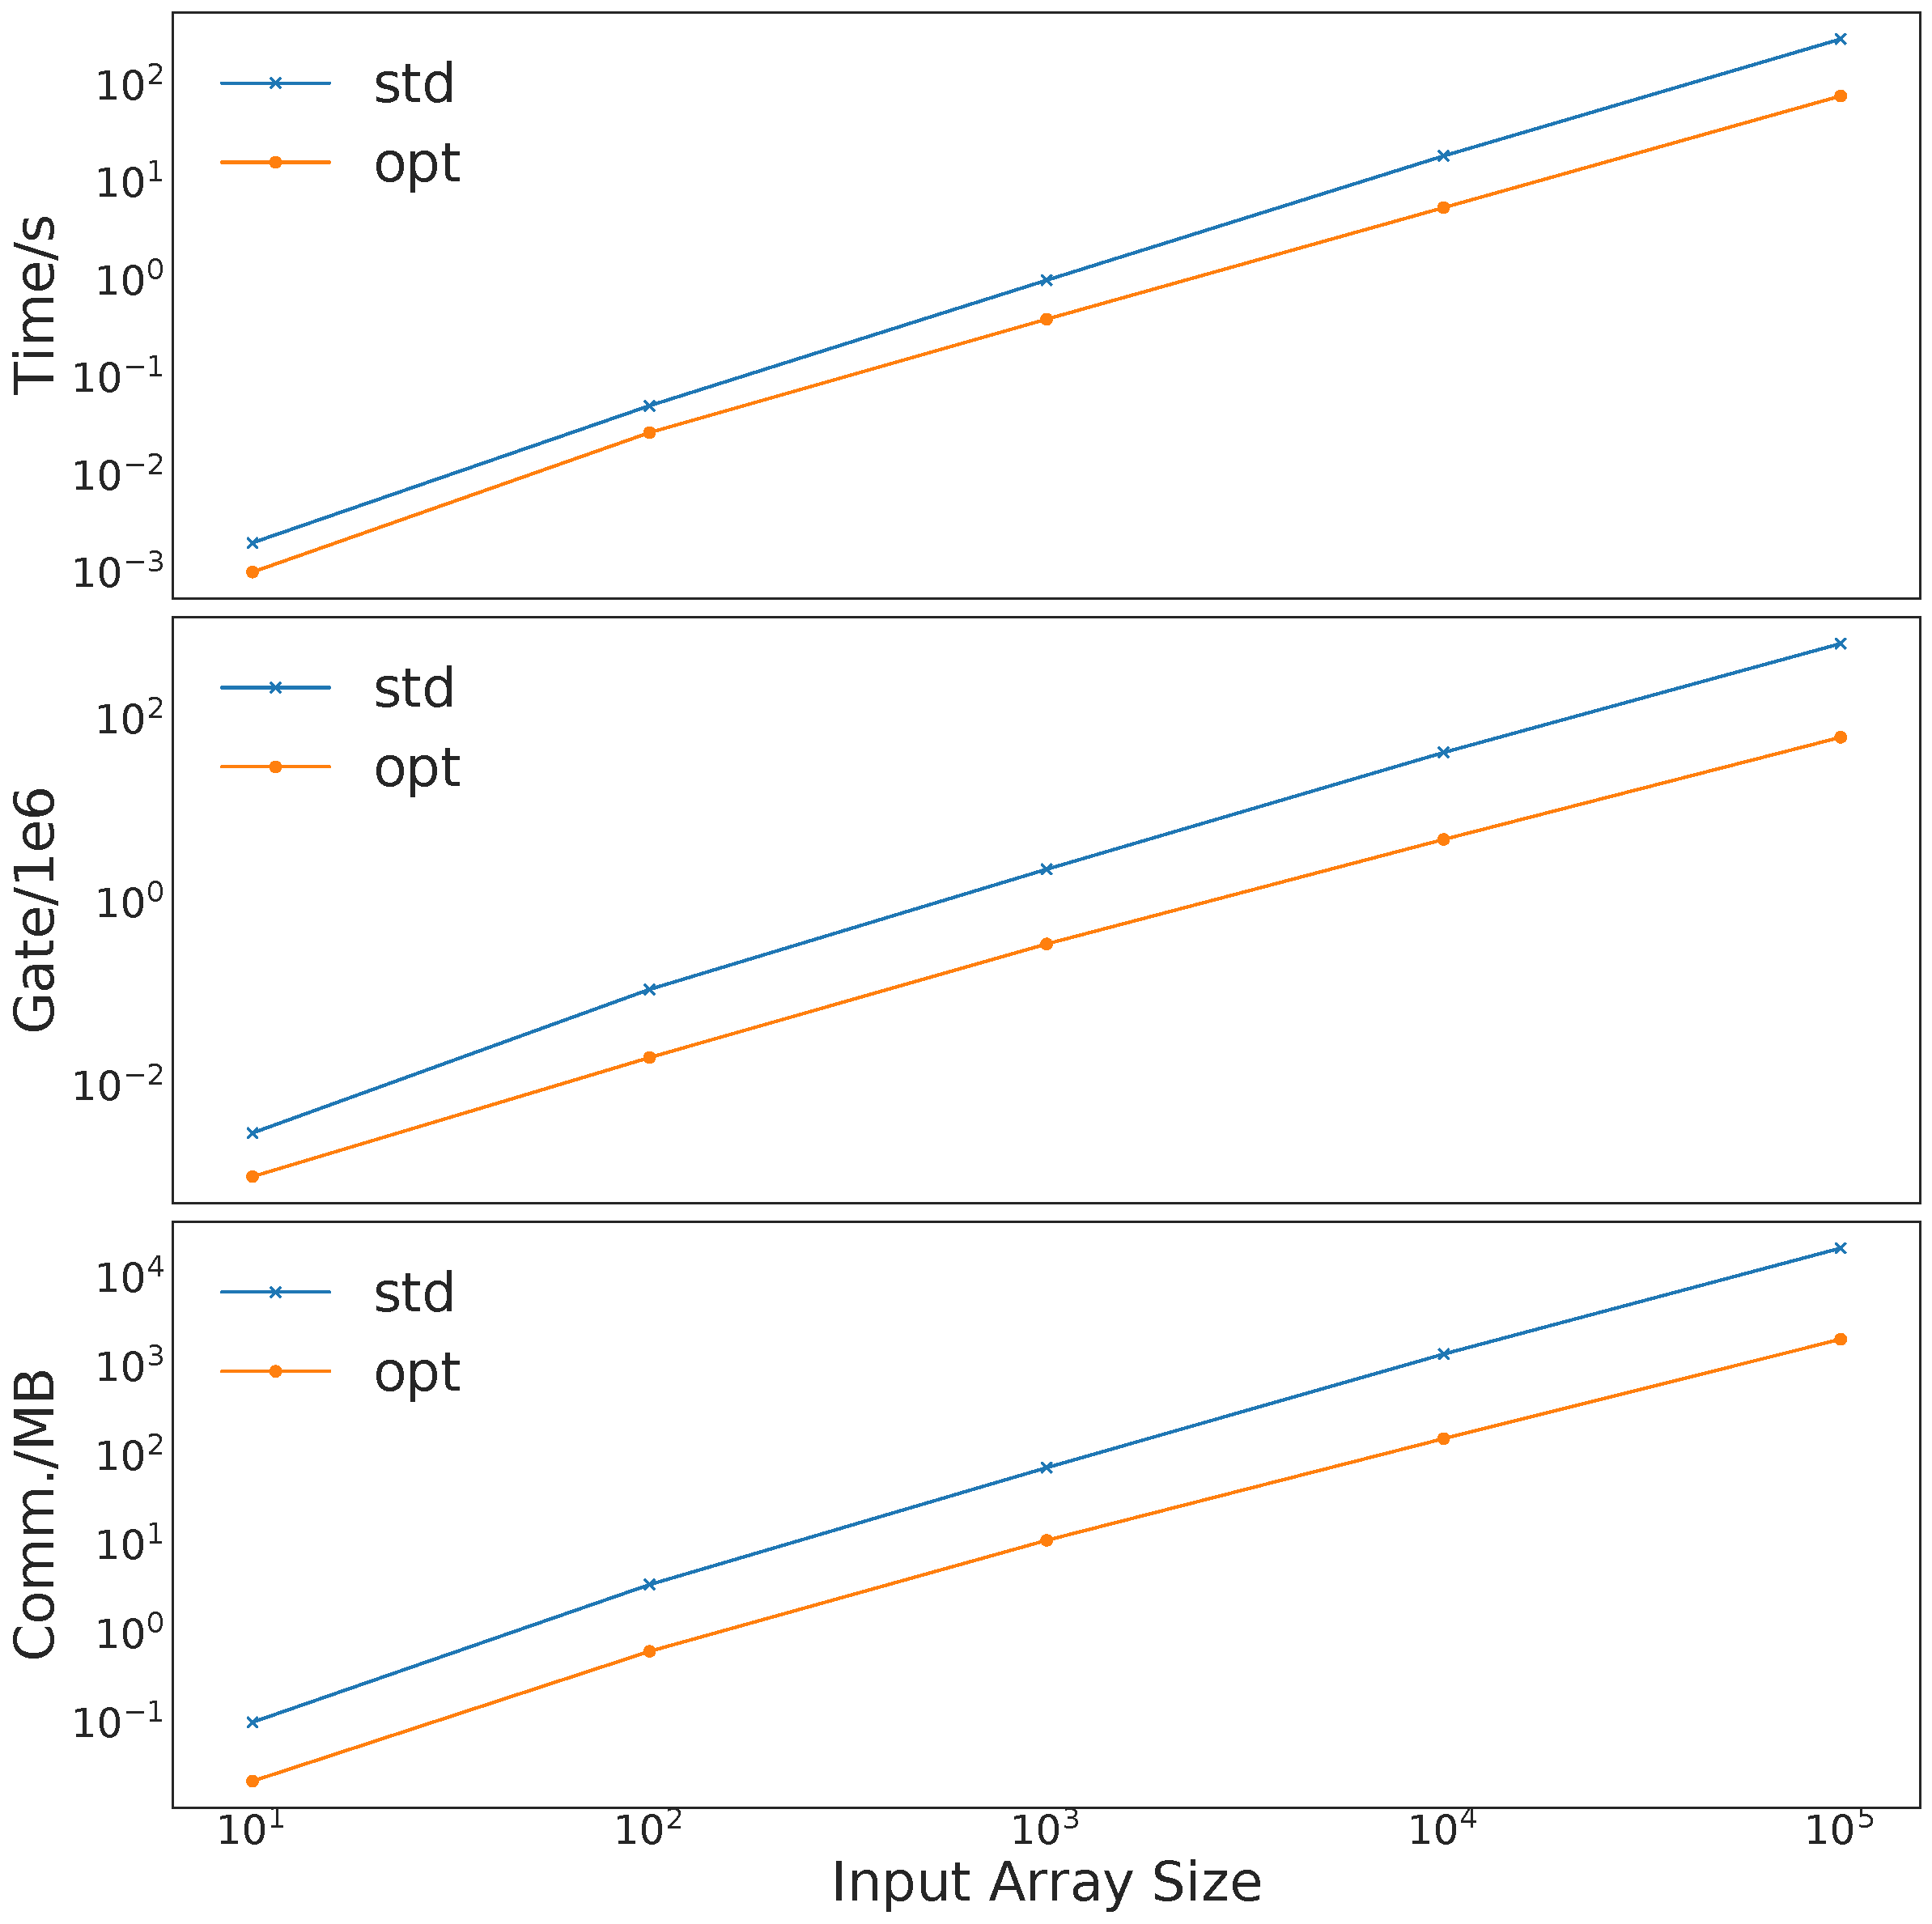
\includegraphics[scale=0.2]{img/gc-sorting.pdf}
    \caption{Communication (Comm.), the number of gates (Gate), protocol execution time (Time) of sorting in Yao's garbled circuit protocol with input array size range from $10^1$ to $10^5$.}
    \label{gcsorting}
\end{figure}
Fig. \ref{gcsorting} shows the performance comparison between sorting std and opt programs in Yao's garbled circuit protocol.

Our opt program reduces 91\% circuit size and communications and achieves 3.84$\times$ speedup.
\begin{figure}[h]
    \centering
    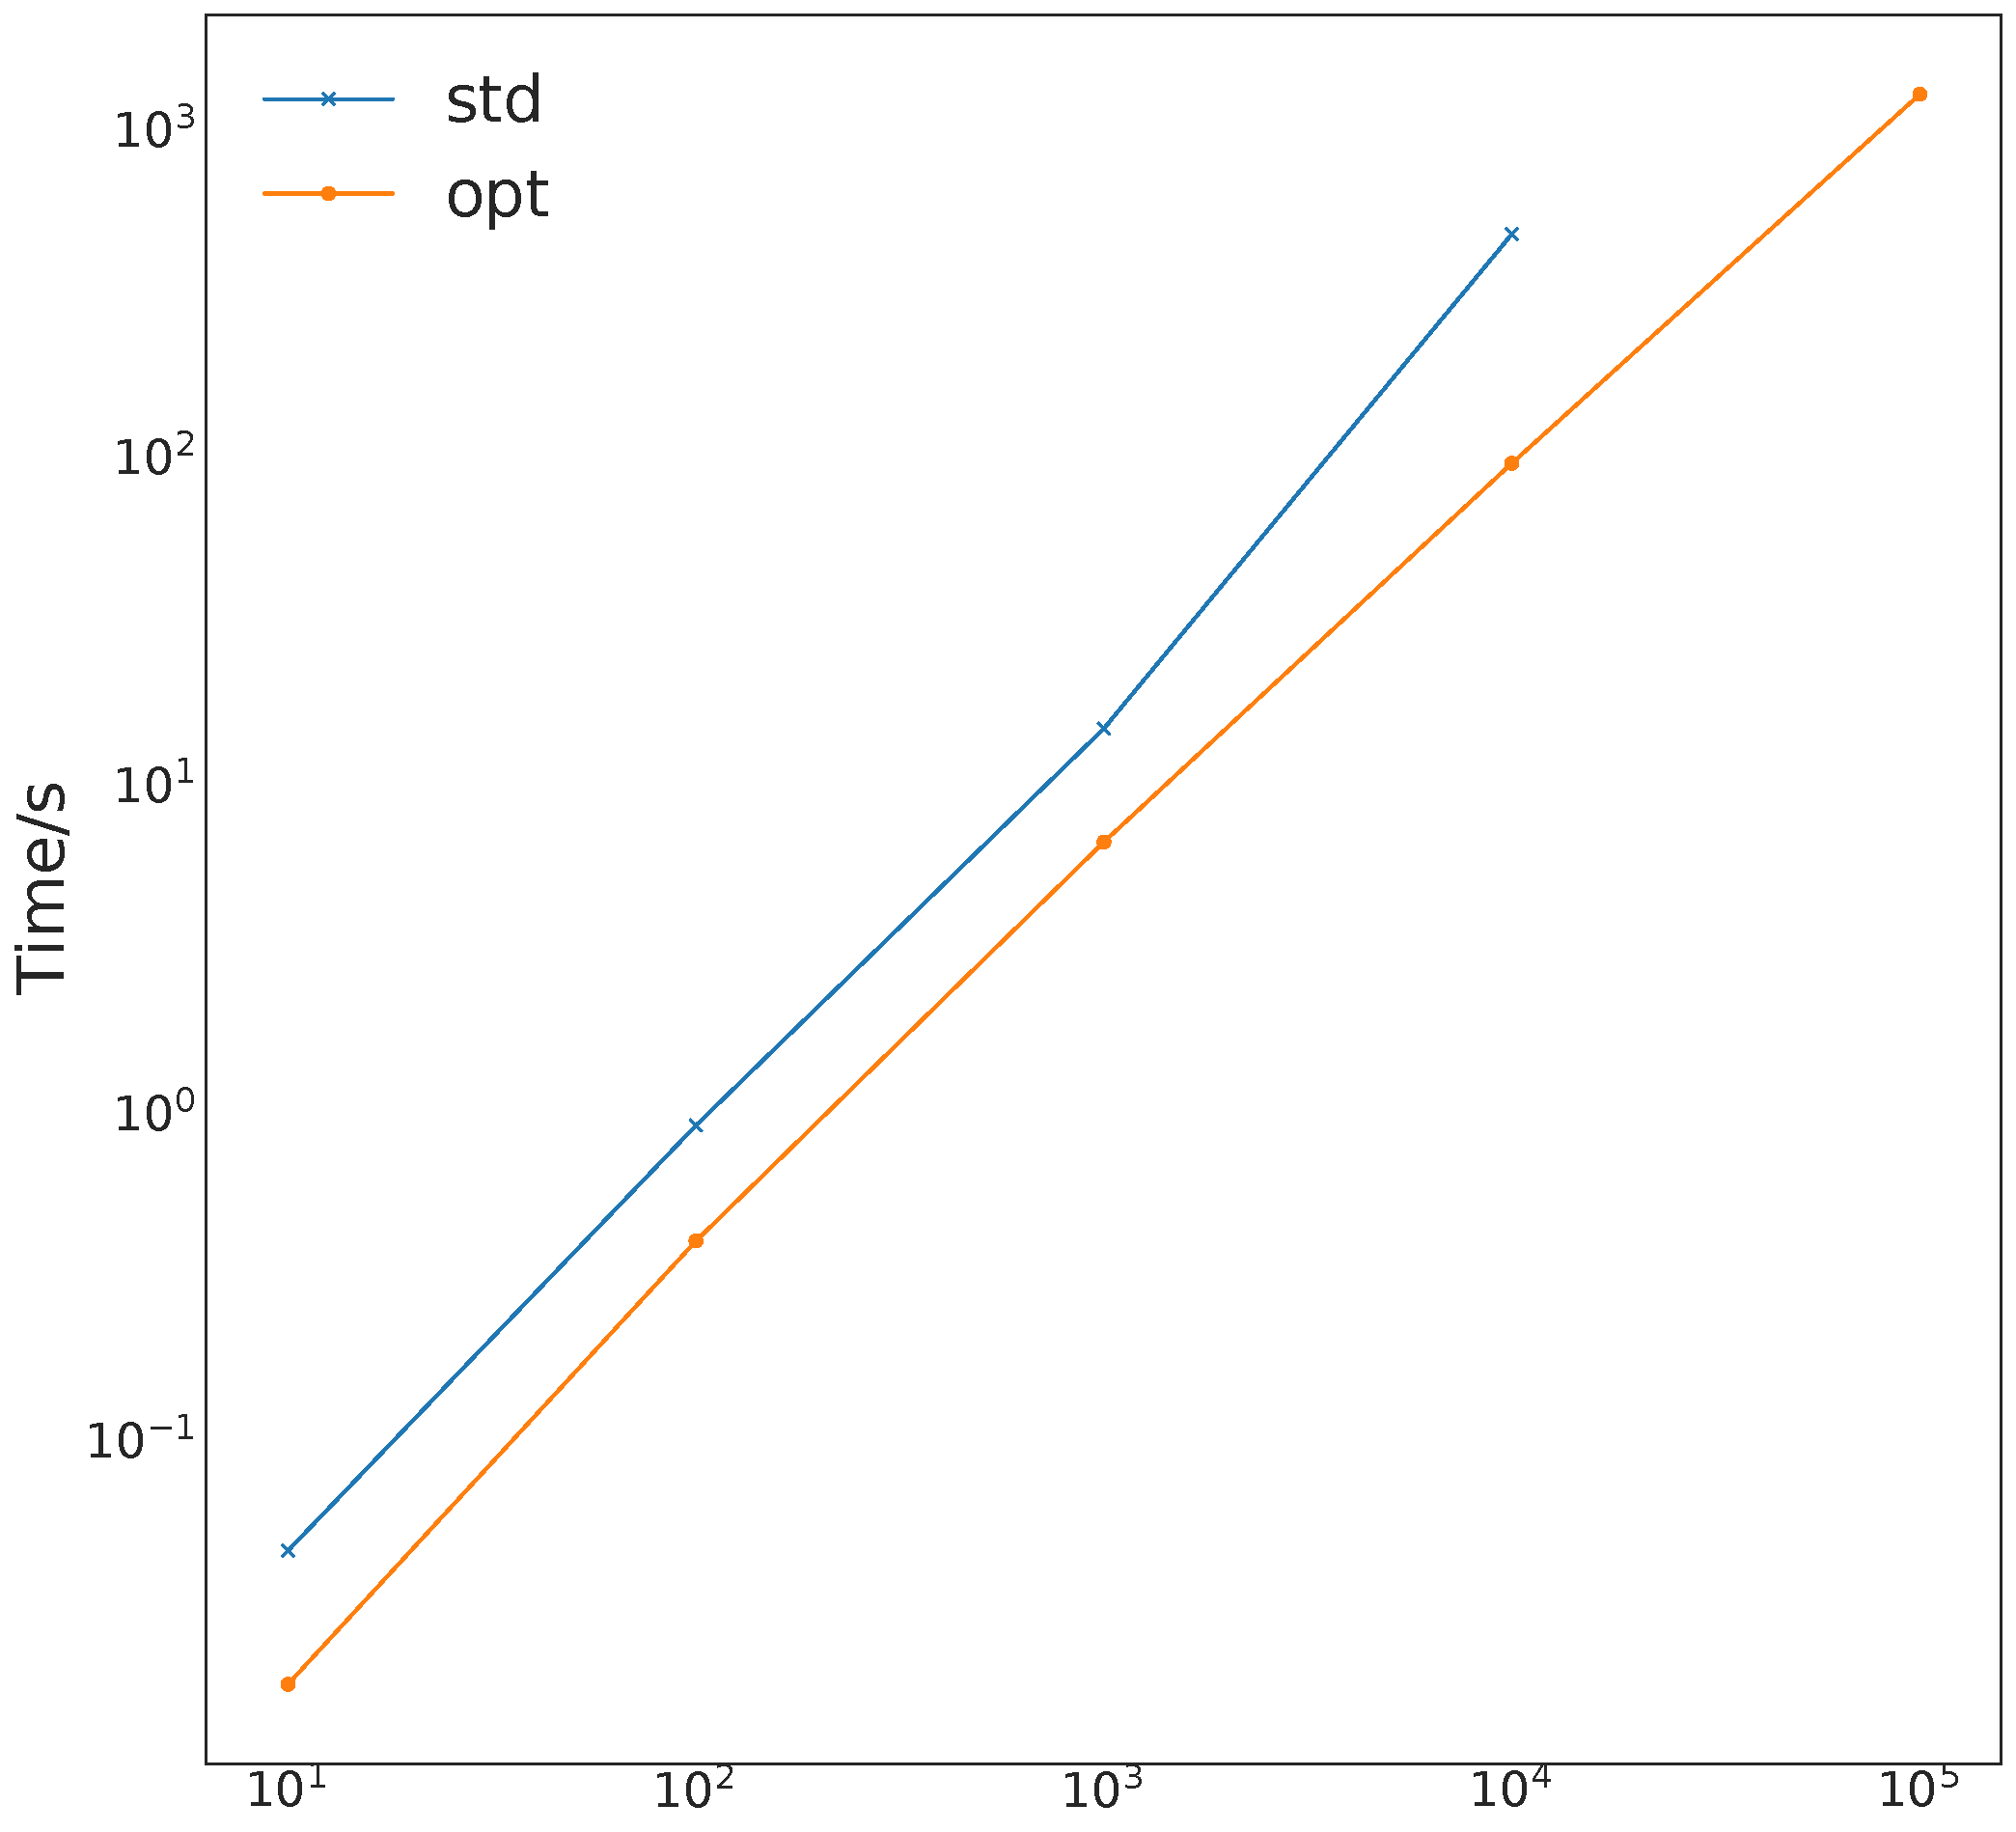
\includegraphics[scale=0.15]{img/ss-sorting.pdf}
    \caption{Performance of sorting in Shamir's secret sharing protocol}
    \label{sssorting}
\end{figure}
In Shamir's secret sharing protocol, our opt program achieves 5.0$\times$ speedup, as shown in Fig. \ref{sssorting}.
\begin{figure}[h]
    \centering
    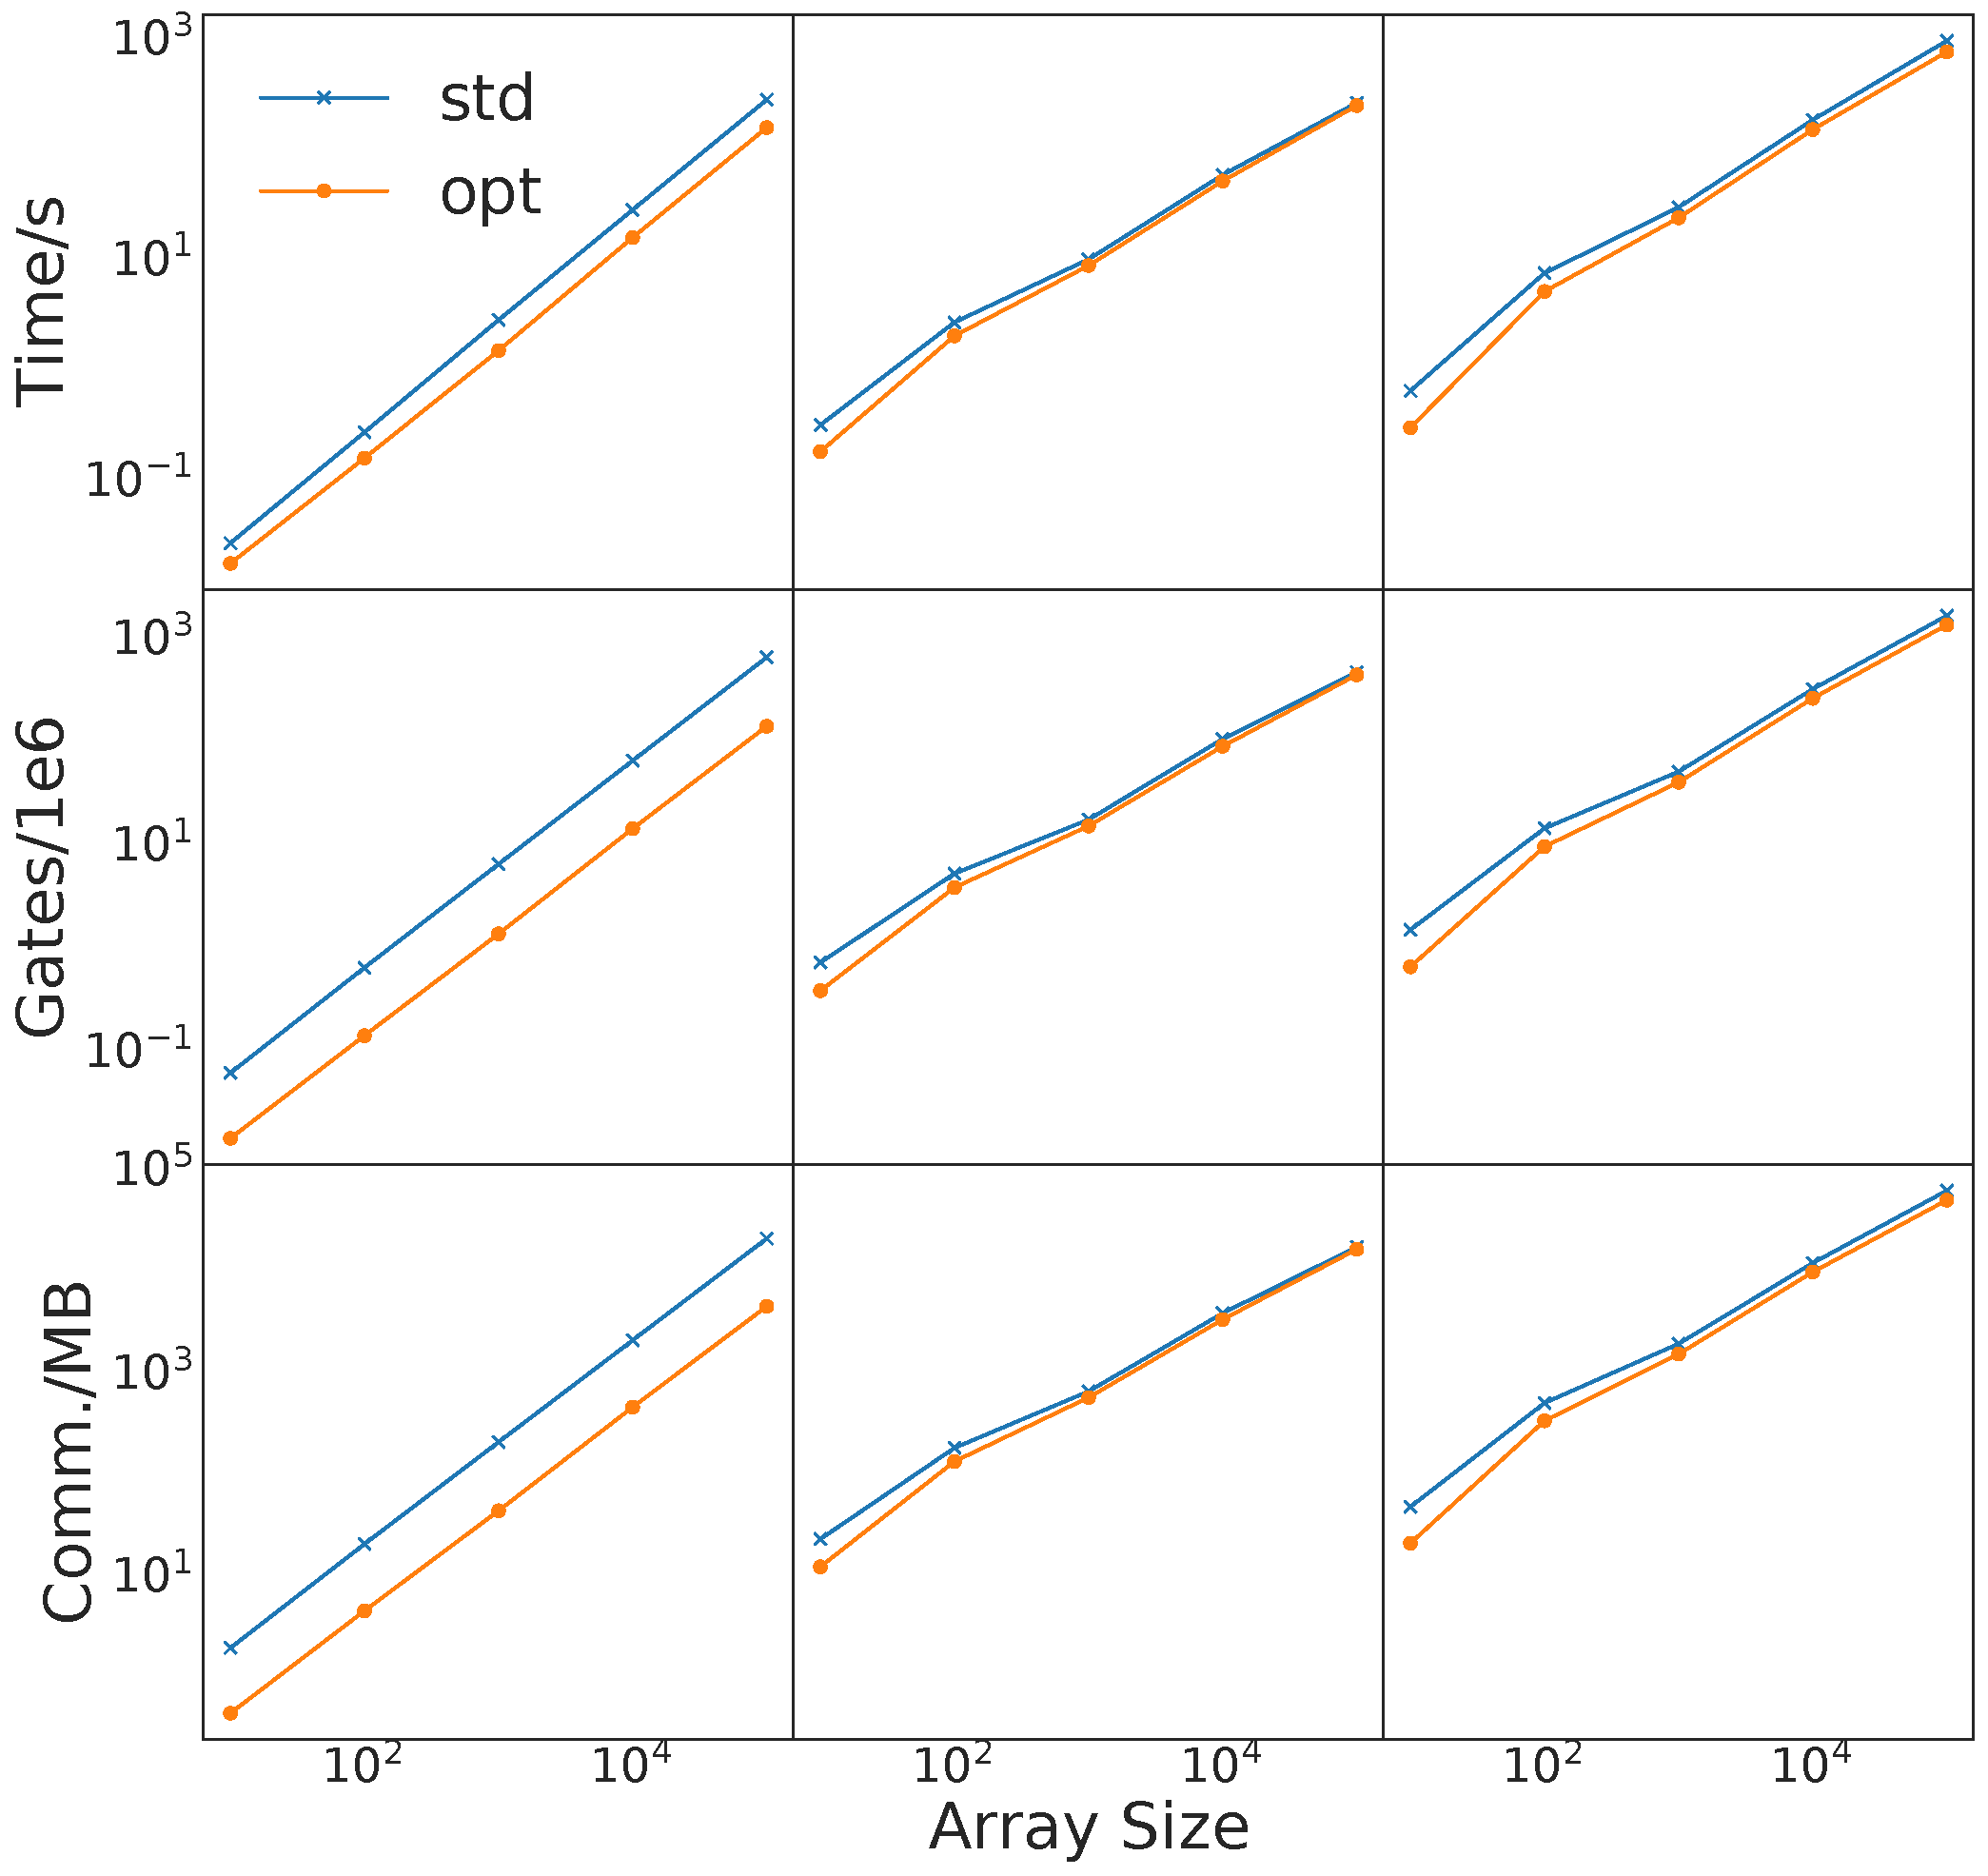
\includegraphics[scale=0.2]{img/gc-search.pdf}
    \caption{Performance of Linear (left), Binary (mid), Almost Search (right) in Yao's garbled circuit protocol}
    \label{gcsearch}
\end{figure}
Our optimization strategy is suitable for different MPC protocols.
From the experiment result, our opt program improves the performance both in Yao's garbled circuit protocol and Secret Sharing protocol.

In this case, the MPC Batcher sort algorithm has $O(n\log^2{n})$ average  time complexity.
With appropriate optimization of the MPC quick sort algorithm, our opt program has  $O(n\log{n})$ average time complexity.
The opt program performs better as the inputs scale increase.

Fig. \ref{gcsearch} shows the performance of three different search study cases in Yao's garbled circuit protocol.
The measurement is searching 100 random elements in the same array.
As array size increases, the performance of opt is reduced because the array size is much larger than 100.
The opt performs better if it searches more elements.
However, our opt program reduces 78\% gates and communications and achieves 1.79$\times$ speedup for linear search.
Binary search work worse than linear search because binary search needs oblivious RAM to access item with secret index.
\begin{figure}[h]
    \centering
    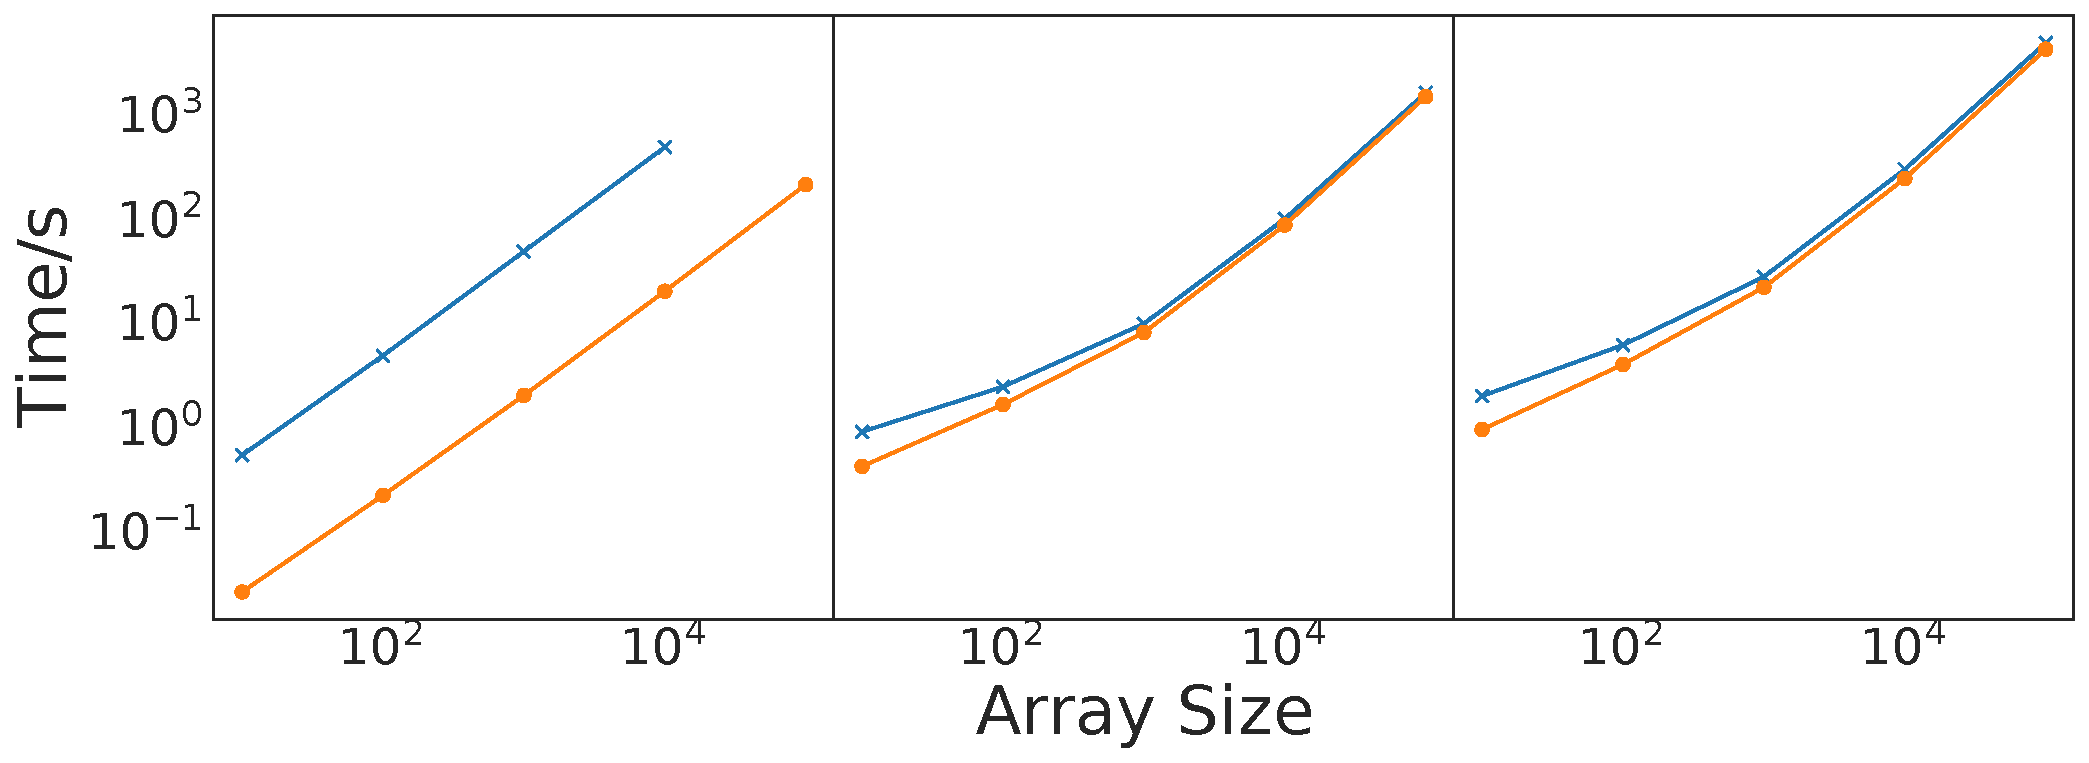
\includegraphics[scale=0.2]{img/ss-search.pdf}
    \caption{Performance of Linear (left), Binary (mid), Almost Search (right) in Shamir's secret sharing protocol}
    \label{sssearch}
\end{figure}
Fig. \ref{sssearch} shows the performance of search study cases in Shamir's secret sharing protocol.
Our opt linear search achieves 24.14$\times$ speedup in 10k array size.
Opt binary search and almost search achieves 1.48$\times$ and 1.54$\times$ speedup when the array size is equal to search size.
The difference of improvement can be explained that Shamir's secret sharing protocol performs not well on comparison operations and oblivious RAM is expensive.

In Yao's garbled circuit protocol, the opt program of line segments intersection reduces 20\% gates and communications and achieves 1.25$\times$ speedup by avoiding calculating coordinates when line segments do not intersect.
The opt program of PSI reduces about 73\% gates and communications and achieves 1.5$\times$ speedup.
In Shamir's secret sharing protocol, the speedup of line intersection and PSI is 1.25$\times$ and 15$\times$.




% \begin{table*}[t]
% \centering
% \setlength{\tabcolsep}{1mm}
% \caption{Execution Time/s of Benchmarks on Garbled Circuit Protocol}
% \begin{tabular}{c|ccccc|ccccc|ccccc}
% \hline
% \multirow{2}{*}{Name} & \multicolumn{5}{c|}{std's input size}       & \multicolumn{5}{c|}{opt's input size}       & \multicolumn{5}{c}{improvement}     \\ \cline{2-16}
%                       & 10    & 100   & 1,000  & 10,000   & 100,000 & 10    & 100   & 1000   & 10000    & 100000  & 10   & 100  & 1000 & 10000 & 100000 \\ \hline
% Sort                  & 0.002 & 0.051 & 0.990  & 18.668   & 295.548 & 0.001 & 0.027 & 0.394  & 5.500    & 77.019  & 50\% & 47\% & 60\% & 71\%  & 74\%   \\ \hline
% Linear Search         & 0.026 & 0.262 & 2.724  & 27.080   & 269.210 & 0.017 & 0.153 & 1.441  & 15.203   & 150.606 & 35\% & 42\% & 47\% & 44\%  & 44\%   \\ \hline
% Binary Search         & 0.305 & 2.595 & 9.662  & 56.205   & 252.489 & 0.175 & 1.958 & 8.477  & 49.390   & 238.511 & 43\% & 25\% & 12\% & 12\%  & 6\%    \\ \hline
% Almost Search         & 0.623 & 7.248 & 28.576 & 176.673  & 919.378 & 0.288 & 4.937 & 22.954 & 144.593  & 729.812 & 54\% & 32\% & 20\% & 18\%  & 21\%   \\ \hline
% Quadratic PSI         & 0.003 & 0.264 & 26.514 & 2647.793 & /       & 0.002 & 0.182 & 17.700 & 1865.526 & /       & 33\% & 31\% & 33\% & 30\%  & /      \\ \hline
% Line Intersection     & 0.284 & 2.642 & 28.723 & 267.920  & /       & 0.216 & 2.273 & 23.350 & 212.480  & /       & 24\% & 14\% & 19\% & 21\%  & /      \\ \hline
% \end{tabular}
% \label{tabgc}%
% \end{table*}

% \begin{table*}[t]
% \centering
% \setlength{\tabcolsep}{1mm}
% \caption{Execution Time/s of Benchmarks on Secret Sharing Protocol}
% \begin{tabular}{c|ccccc|ccccc|ccccc}
% \hline
% \multirow{2}{*}{Name} & \multicolumn{5}{c|}{std's input size}         & \multicolumn{5}{c|}{opt's input size}          & \multicolumn{5}{c}{improvement}     \\ \cline{2-16}
%                       & 10    & 100    & 1,000   & 10,000  & 100,000  & 10    & 100    & 1000    & 10000    & 100000   & 10   & 100  & 1000 & 10000 & 100000 \\ \hline
% Sort                  & 0.046 & 0.912  & 14.817  & 477.358 & /        & 0.018 & 0.405  & 6.677   & 95.459   & 1274.804 & 61\% & 56\% & 55\% & 80\%  & /      \\ \hline
% Linear Search         & 0.534 & 4.821  & 48.126  & 481.939 & /        & 0.026 & 0.220  & 2.001   & 19.966   & 210.700  & 95\% & 95\% & 96\% & 96\%  & /      \\ \hline
% Binary Search         & 0.896 & 2.425  & 9.754   & 99.043  & 1601.835 & 0.417 & 1.637  & 8.025   & 86.270   & 1470.157 & 53\% & 32\% & 18\% & 13\%  & 8\%    \\ \hline
% Almost Search         & 1.975 & 6.087  & 27.509  & 295.545 & 4823.228 & 0.941 & 3.960  & 21.802  & 240.973  & 4195.490 & 52\% & 35\% & 21\% & 18\%  & 13\%   \\ \hline
% Quadratic PSI         & 0.056 & 4.800  & 475.423 & /       & /        & 0.004 & 0.310  & 29.610  & 3216.808 & /        & 93\% & 94\% & 94\% & /     & /      \\ \hline
% Line Intersection     & 3.265 & 32.165 & 320.368 &         &          & 2.688 & 26.416 & 261.388 &          &          & 18\% & 18\% & 18\% & /     & /      \\ \hline
% \end{tabular}
% \label{tabss}%
% \end{table*}

\end{comment}
